% Options for packages loaded elsewhere
% Options for packages loaded elsewhere
\PassOptionsToPackage{unicode}{hyperref}
\PassOptionsToPackage{hyphens}{url}
\PassOptionsToPackage{space}{xeCJK}
%
\documentclass[
  Letterpaper,
]{scrbook}
\usepackage{xcolor}
\usepackage[paperwidth=6in,paperheight=9in]{geometry}
\usepackage{amsmath,amssymb}
\setcounter{secnumdepth}{5}
\usepackage{iftex}
\ifPDFTeX
  \usepackage[T1]{fontenc}
  \usepackage[utf8]{inputenc}
  \usepackage{textcomp} % provide euro and other symbols
\else % if luatex or xetex
  \usepackage{unicode-math} % this also loads fontspec
  \defaultfontfeatures{Scale=MatchLowercase}
  \defaultfontfeatures[\rmfamily]{Ligatures=TeX,Scale=1}
\fi
\usepackage{lmodern}
\ifPDFTeX\else
  % xetex/luatex font selection
  \setmainfont[]{Georgia}
  \ifXeTeX
    \usepackage{xeCJK}
    \setCJKmainfont[]{STSong}
  \fi
  \ifLuaTeX
    \usepackage[]{luatexja-fontspec}
    \setmainjfont[]{STSong}
  \fi
\fi
% Use upquote if available, for straight quotes in verbatim environments
\IfFileExists{upquote.sty}{\usepackage{upquote}}{}
\IfFileExists{microtype.sty}{% use microtype if available
  \usepackage[]{microtype}
  \UseMicrotypeSet[protrusion]{basicmath} % disable protrusion for tt fonts
}{}
\makeatletter
\@ifundefined{KOMAClassName}{% if non-KOMA class
  \IfFileExists{parskip.sty}{%
    \usepackage{parskip}
  }{% else
    \setlength{\parindent}{0pt}
    \setlength{\parskip}{6pt plus 2pt minus 1pt}}
}{% if KOMA class
  \KOMAoptions{parskip=half}}
\makeatother
% Make \paragraph and \subparagraph free-standing
\makeatletter
\ifx\paragraph\undefined\else
  \let\oldparagraph\paragraph
  \renewcommand{\paragraph}{
    \@ifstar
      \xxxParagraphStar
      \xxxParagraphNoStar
  }
  \newcommand{\xxxParagraphStar}[1]{\oldparagraph*{#1}\mbox{}}
  \newcommand{\xxxParagraphNoStar}[1]{\oldparagraph{#1}\mbox{}}
\fi
\ifx\subparagraph\undefined\else
  \let\oldsubparagraph\subparagraph
  \renewcommand{\subparagraph}{
    \@ifstar
      \xxxSubParagraphStar
      \xxxSubParagraphNoStar
  }
  \newcommand{\xxxSubParagraphStar}[1]{\oldsubparagraph*{#1}\mbox{}}
  \newcommand{\xxxSubParagraphNoStar}[1]{\oldsubparagraph{#1}\mbox{}}
\fi
\makeatother


\usepackage{longtable,booktabs,array}
\usepackage{calc} % for calculating minipage widths
% Correct order of tables after \paragraph or \subparagraph
\usepackage{etoolbox}
\makeatletter
\patchcmd\longtable{\par}{\if@noskipsec\mbox{}\fi\par}{}{}
\makeatother
% Allow footnotes in longtable head/foot
\IfFileExists{footnotehyper.sty}{\usepackage{footnotehyper}}{\usepackage{footnote}}
\makesavenoteenv{longtable}
\usepackage{graphicx}
\makeatletter
\newsavebox\pandoc@box
\newcommand*\pandocbounded[1]{% scales image to fit in text height/width
  \sbox\pandoc@box{#1}%
  \Gscale@div\@tempa{\textheight}{\dimexpr\ht\pandoc@box+\dp\pandoc@box\relax}%
  \Gscale@div\@tempb{\linewidth}{\wd\pandoc@box}%
  \ifdim\@tempb\p@<\@tempa\p@\let\@tempa\@tempb\fi% select the smaller of both
  \ifdim\@tempa\p@<\p@\scalebox{\@tempa}{\usebox\pandoc@box}%
  \else\usebox{\pandoc@box}%
  \fi%
}
% Set default figure placement to htbp
\def\fps@figure{htbp}
\makeatother


% definitions for citeproc citations
\NewDocumentCommand\citeproctext{}{}
\NewDocumentCommand\citeproc{mm}{%
  \begingroup\def\citeproctext{#2}\cite{#1}\endgroup}
\makeatletter
 % allow citations to break across lines
 \let\@cite@ofmt\@firstofone
 % avoid brackets around text for \cite:
 \def\@biblabel#1{}
 \def\@cite#1#2{{#1\if@tempswa , #2\fi}}
\makeatother
\newlength{\cslhangindent}
\setlength{\cslhangindent}{1.5em}
\newlength{\csllabelwidth}
\setlength{\csllabelwidth}{3em}
\newenvironment{CSLReferences}[2] % #1 hanging-indent, #2 entry-spacing
 {\begin{list}{}{%
  \setlength{\itemindent}{0pt}
  \setlength{\leftmargin}{0pt}
  \setlength{\parsep}{0pt}
  % turn on hanging indent if param 1 is 1
  \ifodd #1
   \setlength{\leftmargin}{\cslhangindent}
   \setlength{\itemindent}{-1\cslhangindent}
  \fi
  % set entry spacing
  \setlength{\itemsep}{#2\baselineskip}}}
 {\end{list}}
\usepackage{calc}
\newcommand{\CSLBlock}[1]{\hfill\break\parbox[t]{\linewidth}{\strut\ignorespaces#1\strut}}
\newcommand{\CSLLeftMargin}[1]{\parbox[t]{\csllabelwidth}{\strut#1\strut}}
\newcommand{\CSLRightInline}[1]{\parbox[t]{\linewidth - \csllabelwidth}{\strut#1\strut}}
\newcommand{\CSLIndent}[1]{\hspace{\cslhangindent}#1}



\setlength{\emergencystretch}{3em} % prevent overfull lines

\providecommand{\tightlist}{%
  \setlength{\itemsep}{0pt}\setlength{\parskip}{0pt}}



 


\usepackage{xeCJK}
\setCJKmainfont{STSong}
\raggedbottom
\makeatletter
\@ifpackageloaded{tcolorbox}{}{\usepackage[skins,breakable]{tcolorbox}}
\@ifpackageloaded{fontawesome5}{}{\usepackage{fontawesome5}}
\definecolor{quarto-callout-color}{HTML}{909090}
\definecolor{quarto-callout-note-color}{HTML}{0758E5}
\definecolor{quarto-callout-important-color}{HTML}{CC1914}
\definecolor{quarto-callout-warning-color}{HTML}{EB9113}
\definecolor{quarto-callout-tip-color}{HTML}{00A047}
\definecolor{quarto-callout-caution-color}{HTML}{FC5300}
\definecolor{quarto-callout-color-frame}{HTML}{acacac}
\definecolor{quarto-callout-note-color-frame}{HTML}{4582ec}
\definecolor{quarto-callout-important-color-frame}{HTML}{d9534f}
\definecolor{quarto-callout-warning-color-frame}{HTML}{f0ad4e}
\definecolor{quarto-callout-tip-color-frame}{HTML}{02b875}
\definecolor{quarto-callout-caution-color-frame}{HTML}{fd7e14}
\makeatother
\makeatletter
\@ifpackageloaded{bookmark}{}{\usepackage{bookmark}}
\makeatother
\makeatletter
\@ifpackageloaded{caption}{}{\usepackage{caption}}
\AtBeginDocument{%
\ifdefined\contentsname
  \renewcommand*\contentsname{Table of contents}
\else
  \newcommand\contentsname{Table of contents}
\fi
\ifdefined\listfigurename
  \renewcommand*\listfigurename{List of Figures}
\else
  \newcommand\listfigurename{List of Figures}
\fi
\ifdefined\listtablename
  \renewcommand*\listtablename{List of Tables}
\else
  \newcommand\listtablename{List of Tables}
\fi
\ifdefined\figurename
  \renewcommand*\figurename{Figure}
\else
  \newcommand\figurename{Figure}
\fi
\ifdefined\tablename
  \renewcommand*\tablename{Table}
\else
  \newcommand\tablename{Table}
\fi
}
\@ifpackageloaded{float}{}{\usepackage{float}}
\floatstyle{ruled}
\@ifundefined{c@chapter}{\newfloat{codelisting}{h}{lop}}{\newfloat{codelisting}{h}{lop}[chapter]}
\floatname{codelisting}{Listing}
\newcommand*\listoflistings{\listof{codelisting}{List of Listings}}
\makeatother
\makeatletter
\makeatother
\makeatletter
\@ifpackageloaded{caption}{}{\usepackage{caption}}
\@ifpackageloaded{subcaption}{}{\usepackage{subcaption}}
\makeatother
\usepackage{bookmark}
\IfFileExists{xurl.sty}{\usepackage{xurl}}{} % add URL line breaks if available
\urlstyle{same}
\hypersetup{
  pdftitle={The Dictionary Maker},
  pdfauthor={Bude Sethaputra-Piccin},
  hidelinks,
  pdfcreator={LaTeX via pandoc}}


\title{The Dictionary Maker}
\author{Bude Sethaputra-Piccin}
\date{2025-07-24}
\begin{document}
\frontmatter
\maketitle

\renewcommand*\contentsname{Table of contents}
{
\setcounter{tocdepth}{1}
\tableofcontents
}

\mainmatter
\bookmarksetup{startatroot}

\chapter*{Preface}\label{preface}
\addcontentsline{toc}{chapter}{Preface}

\markboth{Preface}{Preface}

In 1933, So Sethaputra was Thailand's youngest Royal Spokesman, a
brilliant Oxford-educated intellectual at the pinnacle of Siamese
society. By 1934, he was Prisoner Number 26 in Bang Kwang prison,
condemned as an enemy of the state following the revolutionary
government's consolidation of power. What happened next defies belief.

During eleven years of imprisonment---first in Bangkok's notorious Bang
Kwang prison, then on the remote islands of Tarutao and Koh Tao---So
accomplished something extraordinary. Working in secret, often by
candlelight, he created Thailand's first comprehensive English-Thai
dictionary. This wasn't merely a translation tool but a cultural bridge
that would educate generations of Thai students and remain influential
decades after its 1949 publication.

\emph{The Dictionary Maker} tells the untold story of intellectual
resistance against authoritarianism, revealing how one man's commitment
to education and cross-cultural understanding transcended political
persecution. Drawing from family archives and historical records, this
account illuminates a crucial period in Thai history when
Western-educated elites faced systematic persecution, yet some found
ways to contribute to their nation's cultural development despite
imprisonment.

As So's granddaughter, I felt compelled to share this remarkable story
of resilience, scholarship, and the transformative power of education.
In our current era of political upheaval and cultural division, So
Sethaputra's example reminds us that intellectual dedication can triumph
over oppression, and that knowledge, once created, becomes an
indestructible gift to future generations.

--- Bude Sethaputra-Piccin

\begin{tcolorbox}[enhanced jigsaw, toprule=.15mm, left=2mm, colback=white, breakable, coltitle=black, bottomrule=.15mm, titlerule=0mm, opacityback=0, bottomtitle=1mm, toptitle=1mm, colbacktitle=quarto-callout-note-color!10!white, title=\textcolor{quarto-callout-note-color}{\faInfo}\hspace{0.5em}{About This Book}, colframe=quarto-callout-note-color-frame, leftrule=.75mm, opacitybacktitle=0.6, rightrule=.15mm, arc=.35mm]

This book was created using the Proofbound CC Template CLI tool. To
learn more about Proofbound visit \url{https://proofbound.com}.

\end{tcolorbox}

\bookmarksetup{startatroot}

\chapter{The Last Siamese}\label{sec-last-siamese}

\section{A Man Between Two Worlds}\label{a-man-between-two-worlds}

So Sethaputra represented the last generation of the old Siamese
elite---Western-educated royalists who witnessed their world disappear
in revolution, war, and social upheaval.

\begin{figure}[H]

{\centering \pandocbounded{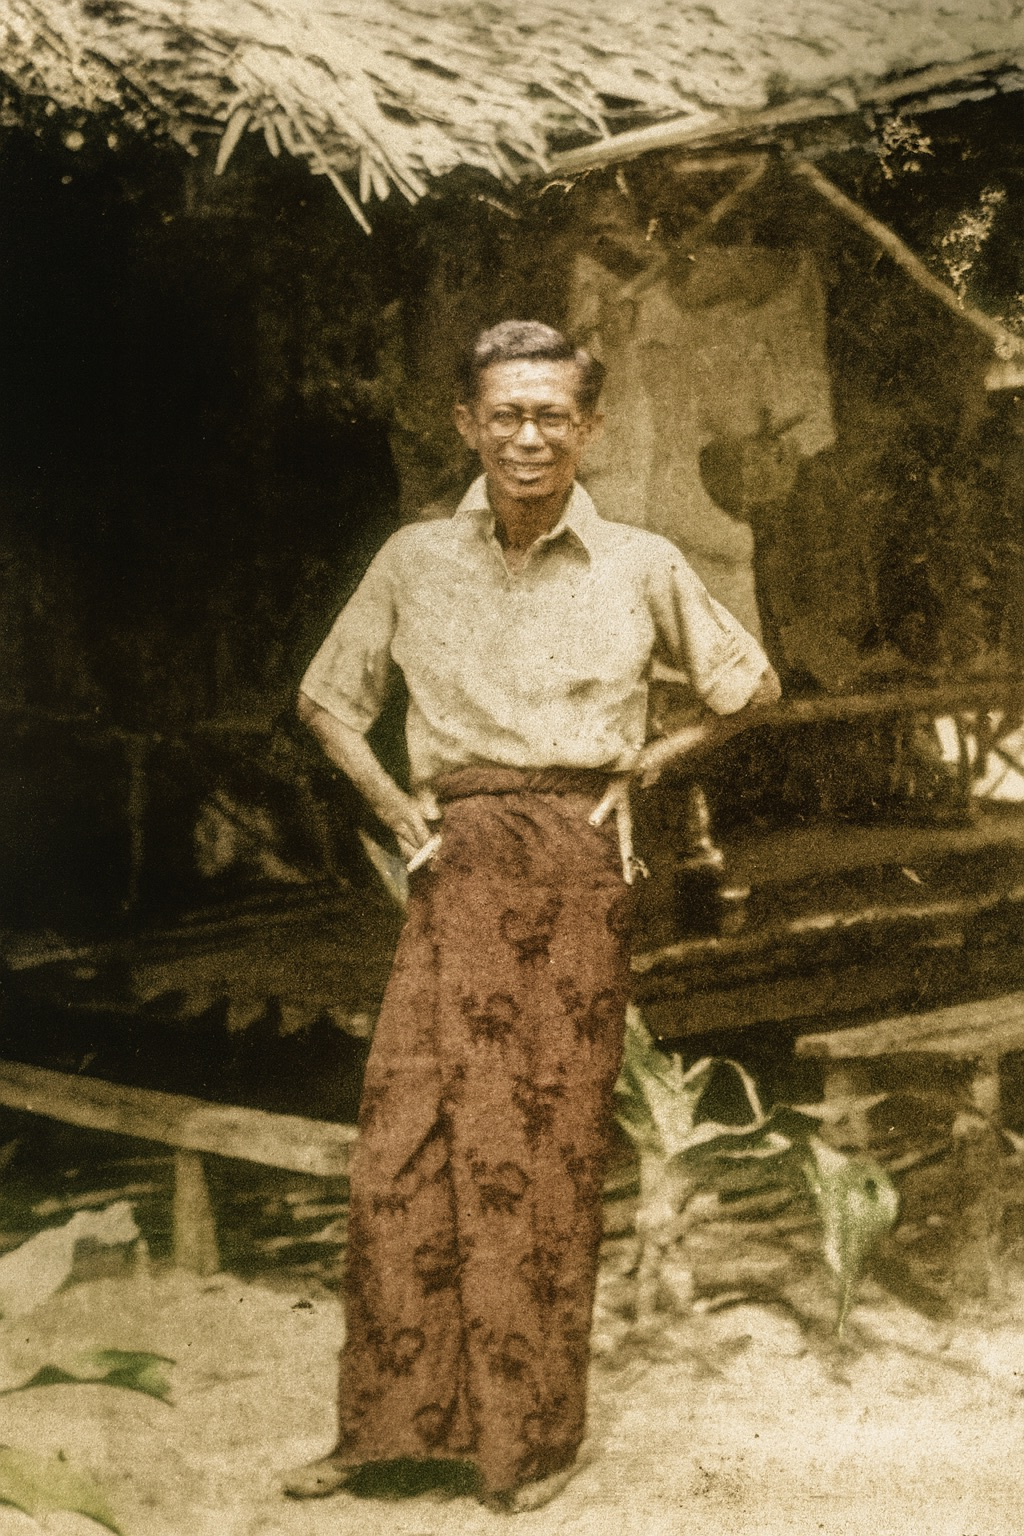
\includegraphics[keepaspectratio]{../_resources/assets/images/ch1-SoSethaputra1.jpeg}}

}

\caption{Sor was always well groomed on Tarutao island, where he served
part of his sentence from 1939 to 1943}

\end{figure}%

In the photograph, So Sethaputra stands with quiet dignity on the remote
prison island of Tarutao, his white shirt immaculately pressed despite
years of confinement, his hair carefully combed, his bearing
unmistakably that of a gentleman. Even in exile, even as Prisoner Number
26, he maintained the composure and refinement that marked him as a
product of old Siam's educated elite. This was a man who refused to let
circumstances diminish his sense of self---a characteristic that would
prove essential to his survival and to the completion of his life's
work.

Born in 1903 into a world that seemed as permanent as the golden spires
of the Grand Palace, So Sethaputra was shaped by the confidence and
cultural certainty of late-nineteenth-century Siam. His was a Thailand
that still called itself by its ancient name, a kingdom that had
successfully navigated the treacherous waters of European colonialism
while preserving its independence and dignity. The Siam of So's youth
was a society in transition, cautiously embracing modernity while
jealously guarding its traditions---much like So himself would do
throughout his extraordinary life.

\section{The Inheritance of Two
Worlds}\label{the-inheritance-of-two-worlds}

So's family embodied the intellectual flowering of late Siamese society.
His father was ``an inquisitive scientist who spent his life inventing
new contraptions,'' a man whose sharp analytical mind and passion for
understanding the natural world would be passed down to his son. In an
era when traditional knowledge systems were encountering Western
scientific methods, So's father represented the bridge between
worlds---a Siamese intellectual who could appreciate both the wisdom of
the ancestors and the discoveries of European science.

But it was from his mother, Gaysorn, that So inherited perhaps his most
crucial gifts: a love of language, literature, and the written word. In
a society where female literacy was still uncommon, Gaysorn was ``one of
the few Siamese women at the turn of the last century who could read and
write.'' This was no small achievement in traditional Siam, where
education had long been the preserve of men and the monastic community.
Her ability to navigate the world of letters made her exceptional, and
she would use this gift not merely for her own enrichment but to become
the invisible co-author of her son's greatest work.

From his mother, So ``developed a passion for literature, books and
writing''---a passion that would sustain him through the darkest years
of his imprisonment. But Gaysorn's influence went far beyond
intellectual inspiration. She was, as So would later write in one of his
dictionary entries, the embodiment of the truth that ``motherly love can
never be destroyed.'' This love would manifest itself in ways that
seemed impossible: smuggling thousands of manuscript pages out of
maximum-security prisons, maintaining a secret correspondence network,
and sustaining her son's work even when the authorities sought to
destroy it.

When So's father died, Gaysorn ``devoted her entire life to him,''
becoming not just a mother but a patron, collaborator, and
co-conspirator. Their relationship would prove to be one of the most
remarkable partnerships in the history of Thai literature---a bond that
transcended the walls of prisons, survived the chaos of war, and
ultimately brought one of Thailand's most important educational works
into existence.

\section{The Last Golden Age}\label{the-last-golden-age}

The Siam of So's youth was a kingdom at the height of its cultural
confidence. Under King Chulalongkorn (Rama V) and his successor King
Vajiravudh (Rama VI), the country had undertaken a remarkable
transformation, modernizing its institutions while preserving its
essential character. This was the era of grand railways and telegraph
lines, of new schools and hospitals, of a bureaucracy increasingly
staffed by merit rather than birth. Yet it was also still recognizably
the Siam of old---a Buddhist kingdom where the monarch was revered as a
semi-divine figure, where court ceremony maintained its ancient
magnificence, and where tradition provided the stable foundation for
progress.

For the educated elite of So's generation, this seemed like the best of
all possible worlds. They could study at European universities---as So
would at a mining engineering program in England---while returning to
positions of honor and influence in a society that valued their
knowledge. They could embrace Western learning without abandoning their
cultural identity, could appreciate Shakespeare and Dickens while
remaining deeply rooted in Thai literature and Buddhist philosophy.

This was a generation that believed in progress without revolution, in
reform without rupture. They saw themselves as the inheritors of a great
civilization that was successfully adapting to the modern world. The
idea that this entire order might be swept away by military coup, that
they might find themselves branded as enemies of the state, would have
seemed not just unlikely but almost inconceivable.

\section{A Mind Shaped by Two
Traditions}\label{a-mind-shaped-by-two-traditions}

So's education followed the pattern typical of his class and generation.
After his foundational schooling in Siam, he traveled to England to
study mining engineering---a practical field that reflected the
kingdom's modernizing ambitions. The choice was not accidental: Siam in
the early twentieth century was eager to develop its natural resources
and reduce its dependence on foreign expertise. Young men like So were
seen as the future leaders who would combine Western technical knowledge
with Thai cultural understanding.

But So's years in England exposed him to more than engineering
principles. He encountered the great traditions of English literature,
became fluent in the language not just as a technical tool but as a
medium of culture and expression. He absorbed the English respect for
democratic institutions, for parliamentary debate, for the gradual
evolution of political systems. When he wrote from England in 1923 that
students in France were ``plotting against the monarchy'' and expressed
his fear that ``they are not interested in democratic change,'' he was
speaking as someone who had come to appreciate the English model of
constitutional development.

Most importantly, his time abroad gave him a comparative perspective on
his own society. He could see Siam's strengths and weaknesses with the
clarity that comes only from distance. He understood that
``parliamentary democracy cannot be instituted by military rule; it is a
gradual learning process, requiring education, experience and good
will.'' This wisdom, gained in the libraries and lecture halls of
England, would inform his later opposition to the hasty and militaristic
changes imposed on his homeland.

\section{The Royal Spokesman}\label{the-royal-spokesman}

When So returned to Siam in 1926, he made a choice that revealed much
about his character and values. Despite his training in mining
engineering, he was ``more interested in journalism'' and ``was a gifted
writer.'' Rather than pursuing the lucrative and prestigious career that
his technical education had prepared him for, he followed his
intellectual passions into the world of media and communication.

His work at the Daily Mail as a political correspondent brought him to
the attention of the highest levels of government. In 1928, ``he was
recognised by his Majesty the King for his communication and language
skills and was appointed Royal Spokesman, today's equivalent of press
secretary.'' This appointment came with the royally-bestowed title of
``Luang Mahasit Woharn''---literally, ``the man of great eloquence.''

The title was more than ceremonial recognition; it reflected So's
genuine gifts as a communicator and his deep understanding of both Thai
and Western cultures. As Royal Spokesman, he served as the bridge
between the ancient institution of the monarchy and the modern world of
journalism and public opinion. He became ``an analyst and adviser on
current diplomatic affairs, foreign trends and local personalities,''
and ``an integral part of the official secretariat of the Royal
household.''

In this role, So was perfectly positioned to understand the tensions and
possibilities of his era. He could see how Thailand was viewed by the
outside world, could gauge the pressures for change that were building
both domestically and internationally. He shared with King Prajadhipok
(Rama VII) the belief ``that a constitutional monarchy supported by a
true democratic parliamentary system would soon prevail in Siam.''

This was the vision of gradual, organic change that appealed to
thoughtful members of the educated elite: reform that would preserve the
best of the old while incorporating the most valuable elements of the
new. It was a vision that required patience, wisdom, and good faith on
all sides---qualities that would prove to be in tragically short supply
when the crisis finally came.

\section{The World That Was Lost}\label{the-world-that-was-lost}

The photograph from Tarutao captures more than just So's personal
dignity; it preserves an image of a vanished world. The man in the white
shirt, maintaining his standards even in prison, represents the last
generation of the old Siamese elite---a class that combined deep
cultural roots with cosmopolitan education, traditional values with
modern knowledge, loyalty to the monarchy with appreciation for
democratic ideals.

These men and women had grown up believing that their society was
successfully navigating the challenges of modernity. They had seen their
kingdom preserve its independence when neighboring Burma, Cambodia,
Laos, and Malaya fell under European control. They had witnessed the
steady development of infrastructure, education, and governance that
seemed to promise continued progress without revolutionary upheaval.

But history had other plans. The military coup of 1932 would shatter
this world as completely as if an earthquake had struck. The patient
work of constitutional reform would be swept aside by the impatience of
junior officers. The gradual evolution toward democracy would be
replaced by the harsh rule of military strongmen. And men like So
Sethaputra---the very people whose education and expertise should have
made them leaders of the new order---would find themselves branded as
enemies and exiled to remote prison islands.

Yet even in defeat, even in exile, So carried within himself the values
and culture of the world he had lost. His insistence on maintaining his
personal dignity, his commitment to education and learning, his belief
in the power of knowledge to transcend political persecution---all of
these reflected the best qualities of the civilization that had shaped
him.

The dictionary he would create in prison was more than a reference work;
it was a preservation of that lost world, a bridge between the Siam that
was and the Thailand that was becoming. In every carefully crafted
definition, in every example sentence drawn from literature and
experience, he was keeping alive the cultural traditions and
intellectual values that the new order seemed determined to destroy.

Standing on Tarutao in his pressed white shirt, So Sethaputra was indeed
``the last Siamese''---not because he was the final representative of an
ethnic group, but because he embodied the spirit of a civilization that
was passing away. His story is the story of that transformation, and of
one man's extraordinary effort to preserve something precious in the
midst of revolutionary change.

\bookmarksetup{startatroot}

\chapter{Siam in Transition}\label{sec-siam-transition}

\section{From Absolute Monarchy to Constitutional
Rule}\label{from-absolute-monarchy-to-constitutional-rule}

The transformation of Siam from an absolute monarchy to a constitutional
system in 1932 marked the end of an era and the beginning of profound
social and political upheaval.

By the 1920s, the kingdom that had shaped So Sethaputra (as described in
Chapter~\ref{sec-last-siamese}) was already showing signs of internal
strain. The confident modernization programs of Kings Chulalongkorn and
Vajiravudh had created new institutions, new classes, and new
expectations that were beginning to challenge the traditional order.
What had seemed like organic evolution was revealing itself to be
revolutionary transformation in disguise.

The Siam of the early twentieth century was a society caught between
worlds. Ancient Buddhist temples stood beside modern government
buildings designed in European architectural styles. Traditional markets
operated in the shadow of new department stores. Rice farmers using
techniques unchanged for centuries worked lands connected to Bangkok by
railways that had reduced journey times from weeks to hours. This was a
kingdom in the midst of perhaps the most rapid transformation in its
long history, yet few recognized how fundamentally the changes would
alter the nature of power and authority.

\section{The Great Transformation}\label{the-great-transformation}

The modernization that began under King Chulalongkorn in the 1870s had
been driven by external necessity. Faced with the colonial expansion of
Britain and France in Southeast Asia, Siam's leaders recognized that
survival required adaptation. The kingdom could preserve its
independence only by demonstrating that it was a modern, civilized state
worthy of respect by European powers. This meant adopting Western-style
administration, legal systems, and educational institutions while
carefully preserving the essential symbols and structures of traditional
authority.

The transformation was remarkable in its scope and speed. Ancient forms
of corvée labor were abolished and replaced with modern taxation
systems. Provincial governors who had ruled like feudal lords were
replaced by salaried civil servants answerable to Bangkok. The
traditional legal system, based on Buddhist principles and customary
law, gave way to codes modeled on European jurisprudence. Most
dramatically, slavery was gradually abolished, freeing hundreds of
thousands of people who had been bound to the land or to noble
households for generations.

These changes created new social dynamics that the monarchy struggled to
control. The new civil service attracted ambitious young men from
families that had never before had access to power. Western education,
initially seen as a tool for strengthening the traditional order, began
to produce graduates who questioned that very order. The introduction of
printing presses and newspapers created public spaces for political
discussion that had never existed in traditional Siam.

By the 1920s, Bangkok had become a cosmopolitan city where traditional
Thai wooden houses stood beside modern concrete buildings, where
Buddhist monks in saffron robes walked streets filled with automobiles,
where traditional shadow puppet performances competed with imported
films from Hollywood. The capital was home to Western-educated
intellectuals, Chinese merchants, European advisors, and a growing
middle class that belonged fully to neither the traditional world nor
the modern one.

\section{The Pressure of New Ideas}\label{the-pressure-of-new-ideas}

The generation of Thai students who went abroad to study in the 1900s
and 1910s returned home with more than technical expertise. They had
absorbed ideas about democracy, nationalism, and popular sovereignty
that were fundamentally incompatible with absolute monarchy. Unlike the
generation that included So Sethaputra, who saw constitutional monarchy
as a natural evolution of traditional kingship, these younger
intellectuals began to question whether monarchy itself was compatible
with modern civilization.

European universities had exposed them to the great political movements
of the age: liberalism, socialism, nationalism, and republicanism. They
had witnessed the dramatic political changes following World War I, when
ancient empires collapsed and new nations emerged based on principles of
popular sovereignty. The Russian Revolution of 1917 had shown that even
the most autocratic regimes could be overthrown by determined
revolutionaries. The Chinese Revolution of 1911 had demonstrated that
Asian societies could successfully adopt republican forms of government.

These ideas fermented in the coffee houses and student organizations of
Bangkok, creating an intellectual underground that grew increasingly
impatient with the pace of political reform. While older intellectuals
like So Sethaputra believed in gradual, organic change that would
preserve the best elements of traditional society, younger radicals saw
the monarchy as an obstacle to genuine modernization.

The tension was particularly acute among military officers, who had been
exposed to Western military organization and doctrine during their
training. They had learned that modern armies were citizens' armies,
motivated by patriotism rather than personal loyalty to a monarch. They
had studied the military reforms that had made Prussia, Japan, and other
nations great powers. Many came to believe that Siam's continued
weakness and dependence on foreign advisors was the direct result of an
outdated political system that concentrated power in the hands of a
traditional elite rather than distributing it among the most capable and
patriotic citizens.

\section{Economic Pressures and Social
Change}\label{economic-pressures-and-social-change}

The global economic crisis that began in 1929 exposed the
vulnerabilities of Siam's modernization program. The kingdom's economy
remained heavily dependent on rice exports, making it vulnerable to
fluctuations in world commodity prices. When rice prices collapsed in
the early 1930s, the government found itself facing a severe fiscal
crisis just as demands for public services and infrastructure investment
were increasing.

The economic pressure fell most heavily on the new middle classes that
had emerged during the modernization period. Government salaries were
cut, public works projects were canceled, and opportunities for
advancement within the bureaucracy became increasingly scarce. Young men
who had invested in Western education found themselves competing for a
shrinking number of positions, while the traditional elite seemed
insulated from the economic hardship by their inherited wealth and
privileged access to the highest levels of government.

The contrast between the government's fiscal austerity and the continued
lavish spending of the royal court became increasingly obvious and
offensive to struggling middle-class families. While civil servants saw
their salaries reduced, the monarchy continued to maintain multiple
palaces, support hundreds of dependents, and fund elaborate ceremonies
that seemed irrelevant to the kingdom's pressing needs.

Rural areas experienced their own forms of economic distress. Peasant
farmers, already burdened by new taxes and increasingly integrated into
a cash economy, found themselves unable to cope with falling crop prices
and rising costs for manufactured goods. Traditional patron-client
relationships that had provided security in times of hardship were being
eroded by the monetization of economic relationships and the
centralization of administrative authority in Bangkok.

The Chinese merchant community, which had grown dramatically during the
modernization period, became a convenient scapegoat for economic
frustrations. Thai nationalism, initially focused on resistance to
European colonial pressure, began to turn inward against internal
minorities. This xenophobic turn would have important political
consequences, as politicians discovered that appeals to ethnic
solidarity could mobilize popular support for radical changes that might
otherwise have been resisted.

\section{The Crisis of Authority}\label{the-crisis-of-authority}

By 1930, the traditional sources of political authority in Siam were
being challenged from multiple directions. The monarchy's claim to rule
by divine right seemed increasingly anachronistic to Western-educated
intellectuals who had absorbed Enlightenment ideas about popular
sovereignty. The traditional nobility's hereditary privileges appeared
unjust to middle-class civil servants who believed that merit rather
than birth should determine access to power. The Buddhist clergy's moral
authority was being questioned by secular intellectuals who saw religion
as an obstacle to scientific progress.

King Prajadhipok, who had ascended to the throne in 1925, was acutely
aware of these pressures. Unlike his predecessors, he had not been
trained from birth to rule and lacked the personal authority that came
from long preparation for kingship. He was intellectually honest enough
to recognize the legitimacy of demands for political reform, but he also
understood the dangers of moving too quickly in dismantling institutions
that had provided stability for centuries.

The king's own inclinations toward constitutional reform created a
paradoxical situation. By acknowledging the need for change, he
inadvertently legitimized more radical demands for transformation. His
willingness to consider limiting royal power was interpreted by some as
weakness and by others as insufficient commitment to genuine democracy.
His careful, gradualist approach satisfied neither conservatives who
wanted to preserve the traditional system nor radicals who demanded
immediate transformation.

The government's handling of the economic crisis further undermined its
authority. Traditional methods of dealing with fiscal problems---raising
taxes and reducing expenditures---seemed inadequate to address the
structural challenges facing the kingdom. The monarchy's response to
popular distress appeared reactive and ineffective, reinforcing
perceptions that the traditional elite were out of touch with the needs
of ordinary citizens.

\section{Intellectual Ferment and Political
Organization}\label{intellectual-ferment-and-political-organization}

The 1920s and early 1930s witnessed an explosion of intellectual and
cultural activity that reflected the kingdom's political tensions. New
magazines and newspapers provided forums for political debate that had
been impossible under the old system of absolute monarchy. Literary
societies, professional organizations, and study groups created spaces
where Western-educated intellectuals could discuss ideas that challenged
traditional assumptions about authority and governance.

The introduction of constitutional monarchy was no longer a question of
whether but when and how. Even conservative intellectuals recognized
that some form of political reform was inevitable. The debate centered
on the pace and extent of change: should transformation be gradual and
evolutionary, preserving as much as possible of the traditional system
while adapting it to modern conditions, or should it be rapid and
revolutionary, sweeping away old institutions to make room for entirely
new forms of organization?

Students returning from Europe brought with them not only new ideas but
also new methods of political organization. They had learned about
political parties, labor unions, professional associations, and other
forms of collective action that were largely unknown in traditional
Siam. Some had participated in student movements and political
organizations in their host countries, gaining practical experience in
modern forms of political mobilization.

These organizational innovations were particularly important in the
military, where young officers began forming secret societies dedicated
to political reform. Unlike civilian intellectuals, who had to rely on
persuasion and public debate, military officers had access to the means
of coercion. Their professional training had taught them to think
strategically about the application of force to achieve political
objectives. Their command of troops gave them the practical capability
to translate ideas into action.

\section{The Moment of Crisis}\label{the-moment-of-crisis}

By 1932, the various pressures that had been building within Siamese
society were approaching a critical point. The economic crisis had
created widespread dissatisfaction with the government's performance.
Intellectual ferment had produced a generation of Western-educated
leaders who were committed to fundamental political change. Military
officers had developed both the ideological commitment and the
organizational capability necessary for revolutionary action.

The traditional elite, including figures like So Sethaputra who would
later pay the price for their loyalty to the old order, remained largely
unaware of how precarious their position had become. They continued to
believe in the possibility of gradual reform that would preserve the
essential features of the monarchical system while adapting it to modern
conditions. This faith in evolutionary change would prove to be their
greatest vulnerability when revolutionary change finally arrived.

The stage was set for the confrontation between old and new that would
transform Siam into Thailand and reshape the lives of an entire
generation. The kingdom that had successfully resisted European
colonization would prove unable to resist the internal pressures
generated by its own modernization program. The confident synthesis of
traditional and modern elements that had characterized the early
twentieth century was about to be shattered by forces that neither the
monarchy nor its loyal servants had anticipated or prepared to resist.

As we shall see in Chapter~\ref{sec-elite-threat}, the Western-educated
intellectuals who had been among the chief beneficiaries of the old
system's modernization program would find themselves among its most
prominent victims when the new order finally emerged. The transformation
of Siam was about to claim its first casualties among those who had done
the most to make it possible.

\bookmarksetup{startatroot}

\chapter{The Elite Under Threat}\label{sec-elite-threat}

\section{Western-Educated Intellectuals in a Changing
World}\label{western-educated-intellectuals-in-a-changing-world}

The Western-educated middle and upper classes of Siam found themselves
caught between loyalty to the old order and the promise of democratic
reform.

While the broader transformation of Siamese society (described in
Chapter~\ref{sec-siam-transition}) created pressures that would
eventually explode into political revolution, its most immediate and
tragic victims would be the very people who had done the most to
modernize the kingdom. The Western-educated elite---men like So
Sethaputra whose story we encountered in
Chapter~\ref{sec-last-siamese}---represented both the greatest
achievement of the old system and its most vulnerable element when the
new order finally emerged.

This was a generation caught in a historical trap of their own making.
Their education and expertise had made them indispensable to the
modernizing monarchy, but their cosmopolitan outlook and commitment to
gradual reform would make them enemies of the revolutionary regime that
replaced it. They had served as bridges between traditional Siam and the
modern world, only to find themselves stranded when the bridge collapsed
beneath them.

\section{The Architecture of Elite
Society}\label{the-architecture-of-elite-society}

The Western-educated elite of early twentieth-century Siam represented a
remarkable social experiment. Unlike the traditional nobility, whose
authority derived from birth and royal favor, this new class had earned
their positions through merit, education, and service to the crown. They
were the products of King Chulalongkorn's ambitious program to create a
modern administrative class that could compete with European colonial
governments while remaining loyal to Siamese traditions.

The system had worked brilliantly for several decades. Young men from
good families were selected for government scholarships to study in
Europe, where they absorbed Western knowledge while maintaining their
cultural identity as Siamese subjects. They returned home to take
positions in the expanding bureaucracy, bringing technical expertise and
international perspective to the task of modernizing the kingdom. Their
success had validated the monarchy's strategy of controlled
modernization---change that would strengthen rather than threaten
traditional authority.

By the 1920s, this elite had created a distinctive culture that blended
Eastern and Western elements with remarkable sophistication. They lived
in Bangkok neighborhoods where traditional wooden houses had been
renovated with modern conveniences, where English libraries sat
alongside Buddhist shrines, where European furniture was arranged around
traditional Thai art. Their children attended schools that taught both
Thai classical literature and Western science, that emphasized Buddhist
ethics alongside European philosophy.

Their social world revolved around institutions that had no equivalent
in traditional Siam: professional associations, literary societies,
alumni organizations, and charitable foundations. These groups provided
forums for intellectual discussion and cultural exchange that enriched
the kingdom's cultural life while creating networks of shared interest
and mutual obligation. The Royal Bangkok Sports Club, the Siam Society,
and similar organizations became centers of an emerging civil society
that seemed to promise gradual evolution toward constitutional
democracy.

The elite's lifestyle reflected their unique position between worlds.
They might begin their day reading English newspapers over
European-style breakfast, spend their morning in government offices
conducting business in Thai, attend afternoon meetings where they
discussed Western political theory, and end their evening at traditional
cultural performances. Their wardrobes included both Western suits for
official functions and traditional Thai clothing for court ceremonies.
Their libraries contained works by Shakespeare and Dickens alongside
classical Thai poetry and Buddhist texts.

\section{Professional Networks and Intellectual
Communities}\label{professional-networks-and-intellectual-communities}

The Western-educated elite had created an intellectual ecosystem that
was unprecedented in Siamese history. Professional journals published
articles on engineering, medicine, law, and education that reflected
international standards while addressing uniquely Thai concerns.
Literary magazines featured poetry and essays that experimented with
Western forms while drawing on Thai cultural themes. Newspapers provided
sophisticated coverage of both domestic politics and international
affairs, creating an informed public discourse that had been impossible
under the old system of absolute monarchy.

These publications were more than mere vehicles for information; they
were instruments of cultural creation. Through their pages, the
Western-educated elite were literally inventing modern Thai
identity---finding ways to be simultaneously Thai and modern, Buddhist
and scientific, loyal to the monarchy and committed to democratic
principles. Their success in this cultural synthesis was evident in the
quality of their work: Thai literature and journalism of the 1920s
achieved standards that would not be surpassed for decades.

The intellectual networks they created extended beyond national
boundaries. Many maintained correspondence with classmates and
colleagues in Europe, America, and other Asian countries. They attended
international conferences, contributed to foreign publications, and
participated in global conversations about modernization, nationalism,
and political development. This cosmopolitan outlook was both their
greatest strength and their greatest vulnerability: it gave them
international perspective and credibility, but it also made them suspect
to more parochial political movements.

Their children represented the ultimate test of their cultural
synthesis. The second generation of Western-educated families were even
more comfortable moving between Thai and international contexts, even
more skilled at combining traditional values with modern knowledge. Many
spoke three or four languages fluently, felt equally at home in Bangkok
and London, and seemed to represent the future of a Thailand that would
be both authentically Asian and fully modern.

\section{The Economic Foundation of Elite
Status}\label{the-economic-foundation-of-elite-status}

The Western-educated elite's position in society was secured not only by
their education and expertise but also by their economic circumstances.
Most had achieved a level of prosperity that was modest by European
standards but substantial within the Siamese context. Their salaries as
government officials, supplemented by private consulting work and
investments, allowed them to maintain households that included servants,
automobiles, and other markers of modern middle-class status.

Their economic security was built on assumptions about the stability and
growth of the modernizing Siamese state. They had invested in education
for their children, in property in Bangkok's expanding suburbs, in
businesses that served the growing modern sector of the economy. Their
prosperity depended on continued political stability and the ongoing
integration of Siam into the global economy. They were, in effect,
betting their futures on the success of the modernization program they
were helping to implement.

This economic foundation created both confidence and vulnerability.
Their prosperity allowed them to take intellectual risks, to experiment
with new ideas, to maintain the independence of thought that made them
valuable advisors to the monarchy. But it also made them dependent on
the continued favor of the political system that employed them. Unlike
traditional nobles, who owned land and maintained private armies, the
Western-educated elite possessed only their expertise and their
reputations. If the political winds shifted, they had few resources with
which to protect themselves.

The global economic crisis that began in 1929 exposed the fragility of
their position. Government salaries were reduced, private consulting
opportunities disappeared, and investment values collapsed. For the
first time since the beginning of the modernization program, many
members of the Western-educated elite found themselves facing genuine
economic hardship. Their children's education was threatened, their
standard of living declined, and their confidence in the future was
shaken.

\section{Cultural Leadership and Public
Service}\label{cultural-leadership-and-public-service}

Despite their relatively small numbers---perhaps a few thousand
individuals in a population of millions---the Western-educated elite
exercised influence far beyond their demographic weight. They dominated
the higher levels of government administration, provided leadership for
cultural and educational institutions, and served as interpreters
between Siam and the outside world. Their opinions carried weight not
only because of their official positions but because of their
demonstrated competence and their commitment to public service.

Their approach to cultural leadership reflected their synthesis of
Eastern and Western values. They promoted traditional Thai arts while
introducing Western aesthetic concepts. They supported Buddhist
institutions while advocating for scientific education. They celebrated
Siamese history while working to modernize Siamese society. This
balanced approach had broad appeal and seemed to point toward a future
in which Thailand could be both authentically itself and successfully
modern.

Their commitment to public service distinguished them from both
traditional nobles, who often viewed government positions as sources of
personal enrichment, and from purely Western-trained technocrats, who
might lack understanding of local conditions and values. They brought to
their work a combination of technical competence and cultural
sensitivity that made them exceptionally effective administrators and
advisors.

Many supplemented their official duties with voluntary work in
education, healthcare, and social welfare. They founded schools,
hospitals, and charitable organizations that served broader public needs
while demonstrating their commitment to social progress. Their example
helped establish traditions of civic engagement and philanthropic
activity that would survive the political upheavals that destroyed their
own class position.

\section{The Growing Isolation}\label{the-growing-isolation}

By the early 1930s, however, the Western-educated elite were becoming
increasingly isolated from broader currents in Siamese society. Their
cosmopolitan outlook and gradual approach to reform put them at odds
with more radical political movements that were gaining momentum among
younger intellectuals and military officers. Their prosperity and
privileged positions made them targets of resentment during the economic
crisis. Their close association with the monarchy made them suspect to
republicans and democrats who saw constitutional reform as insufficient.

The very qualities that had made them successful---their moderation,
their international perspective, their commitment to gradual
change---began to seem like weaknesses in an increasingly polarized
political environment. Radical nationalists viewed their cosmopolitanism
as lack of patriotism. Economic populists saw their prosperity as
evidence of corruption. Military reformers regarded their civilian
expertise as irrelevant to the task of national regeneration.

Their faith in constitutional monarchy as the solution to Siam's
political problems put them in an increasingly untenable position. They
continued to believe that the monarchy could be reformed and
democratized, that traditional institutions could be adapted to modern
conditions, that revolutionary change was both unnecessary and
dangerous. This belief would prove to be both their defining
characteristic and their ultimate downfall.

As we shall see in Chapter~\ref{sec-coup-aftermath}, when the
revolutionary moment finally arrived in June 1932, the Western-educated
elite would find themselves not among the architects of change but among
its victims. Their years of loyal service to the crown, their expertise
in modern administration, their commitment to gradual reform---none of
these would protect them from the revolutionary tide that would sweep
away the world they had worked so hard to create.

The tragedy of their situation was that they represented the best
possibilities of the old system: educated, competent, public-spirited,
and committed to progress. Their destruction would deprive Thailand of
much of its intellectual leadership just at the moment when such
leadership was most desperately needed. In their fall, the kingdom would
lose not only valuable servants but also the possibility of evolutionary
change that might have avoided the traumas and instabilities that would
characterize Thai politics for decades to come.

Among those who would pay the highest price for their loyalty to the old
order was So Sethaputra, whose prison years would become both a personal
catastrophe and an unlikely opportunity to create something of lasting
value for Thai society. His story, which we will follow through the dark
years ahead, illustrates both the tragedy of his generation and its
remarkable capacity for intellectual courage under the most difficult
circumstances.

\bookmarksetup{startatroot}

\chapter{The Coup and Its Aftermath}\label{sec-coup-aftermath}

\section{June 24, 1932: The End of Absolute
Monarchy}\label{june-24-1932-the-end-of-absolute-monarchy}

The bloodless coup that ended Thailand's absolute monarchy set in motion
events that would transform the kingdom and seal So Sethaputra's fate.

At dawn on June 24, 1932, the world that had shaped So Sethaputra and
his generation (described in Chapter~\ref{sec-last-siamese}) came to an
abrupt end. The Western-educated elite who had served as bridges between
traditional and modern Siam (as examined in
Chapter~\ref{sec-elite-threat}) suddenly found themselves not among the
architects of change but among its most prominent victims. The
revolutionary transformation that had been building pressure within
Siamese society (outlined in Chapter~\ref{sec-siam-transition}) finally
exploded into action with a precision and audacity that caught the
traditional establishment completely off guard.

The conspirators who gathered in the pre-dawn darkness of Bangkok were
not the gradualist reformers who had dominated intellectual discourse
for decades. They were a new breed of political actors: young military
officers and civilian intellectuals who had grown impatient with the
monarchy's cautious approach to constitutional reform. Led by figures
who would reshape Thai politics for generations, they represented the
triumph of revolutionary over evolutionary change.

\section{The Revolutionaries and Their
Vision}\label{the-revolutionaries-and-their-vision}

The coup was the work of a secret organization called the People's
Party, founded in Paris in 1927 by Thai students and military officers
studying in Europe. Unlike the established elite who believed in working
within existing institutions, these conspirators had concluded that
fundamental change required the complete overthrow of the absolute
monarchy. They had watched the gradual reforms of the 1920s with growing
frustration, convinced that the traditional elite would never
voluntarily surrender their privileged position.

The People's Party's leadership reflected the new political dynamics
that had emerged within Thai society. Military officers predominated,
but the group also included civilian intellectuals who brought
ideological sophistication to the revolutionary enterprise. What united
them was not a detailed program for governing Thailand but a shared
conviction that absolute monarchy was incompatible with modern
nationhood.

Their ideology was a complex mixture of nationalism, democracy, and
socialism that reflected the intellectual ferment of 1920s Europe. They
had absorbed ideas from the Russian Revolution, from European social
democratic movements, and from emerging theories of anti-colonial
nationalism. Their vision for Thailand emphasized popular sovereignty,
economic development, and national independence from foreign influence.
Most importantly, they believed that revolutionary change was both
necessary and urgent.

The contrast with the established elite could not have been more stark.
While figures like So Sethaputra believed that ``parliamentary democracy
cannot be instituted by military rule; it is a gradual learning process,
requiring education, experience and good will,'' the revolutionaries
were convinced that only decisive action could break the grip of
traditional privilege. They saw patience as weakness, compromise as
betrayal, and gradualism as a strategy for preventing real change.

\section{The Morning That Changed
Everything}\label{the-morning-that-changed-everything}

The coup itself was executed with remarkable precision. A small group of
tanks and artillery pieces were positioned around key government
buildings in Bangkok, while coordinated groups of officers secured
strategic points throughout the capital. The operation was designed to
present the monarchy and its supporters with a fait accompli: the
absolute monarchy had been abolished, and resistance would be futile.

King Prajadhipok, who had spent months considering various proposals for
constitutional reform, awoke to discover that the decision had been
taken out of his hands. The revolutionaries presented him with an
ultimatum: accept the new constitutional order or face the consequences
of resistance. Isolated from his traditional supporters and confronted
with the reality of military force, the king had little choice but to
acquiesce.

The coup's success owed much to the political isolation of the
traditional elite. The Western-educated intellectuals who might have
provided leadership for a counter-revolutionary response were scattered
and unprepared. Many were traveling abroad, others were caught up in
their academic and professional pursuits, and still others simply could
not believe that such a dramatic transformation was possible. The very
qualities that had made them effective administrators---their
deliberative approach to problems, their faith in institutional
solutions, their belief in gradual change---rendered them helpless in
the face of revolutionary action.

The traditional nobility fared no better. Accustomed to operating
through court intrigue and personal relationships with the monarch, they
found themselves irrelevant in a political system that had suddenly been
transformed. Their wealth and social connections, which had provided
security for generations, offered no protection against determined
revolutionaries with clear political objectives and military support.

\section{The New Order's
Consolidation}\label{the-new-orders-consolidation}

The revolutionaries moved quickly to consolidate their victory and
eliminate potential sources of opposition. New laws were promulgated
that dramatically expanded the definition of political crimes, making
virtually any criticism of the new order potentially treasonous. The
press, which had enjoyed increasing freedom during the final years of
absolute monarchy, found itself subject to strict censorship. Political
organizations that might serve as focal points for opposition were
banned or subjected to intensive surveillance.

Most ominously for the Western-educated elite, the new government began
a systematic campaign to remove potential opponents from positions of
influence. Senior civil servants who were deemed insufficiently loyal to
the revolutionary cause found themselves transferred to insignificant
posts or forced into early retirement. Military officers who had
maintained close ties to the monarchy were dismissed or placed under
surveillance. Intellectuals who had advocated gradual reform rather than
revolutionary change discovered that their previous service to the crown
was now evidence of counter-revolutionary sentiment.

The speed and thoroughness of these changes reflected the
revolutionaries' understanding that their victory would remain
precarious as long as the old elite retained any capacity for organized
resistance. They had studied successful revolutions in other countries
and understood that half-measures were more dangerous than decisive
action. The traditional elite had to be not merely defeated but
thoroughly demoralized and scattered.

For individuals like So Sethaputra, who had built their careers on loyal
service to the monarchy and belief in constitutional evolution, the new
political environment was both incomprehensible and threatening. Their
expertise in modern administration, their international connections,
their commitment to democratic principles---all of the qualities that
had made them valuable servants of the old order now made them suspect
in the eyes of the new regime.

\section{So Sethaputra's Dilemma}\label{so-sethaputras-dilemma}

So's position as Royal Spokesman made him particularly vulnerable to the
new government's suspicion. His role had required him to defend and
explain royal policies to the press and public, making him a visible
symbol of the monarchical system that the revolutionaries had
overthrown. His eloquence and persuasive abilities, which had once been
assets, now marked him as a potential leader of counter-revolutionary
sentiment.

More fundamentally, So's entire worldview was antithetical to the
revolutionary ideology that now dominated Thai politics. His belief in
gradual reform, his faith in constitutional monarchy, his commitment to
preserving the best elements of traditional culture while adapting to
modern conditions---all of these positions put him at odds with
revolutionaries who saw compromise as weakness and moderation as
betrayal.

So faced the dilemma that confronted all members of his generation:
adapt to the new order by abandoning their principles, or remain true to
their beliefs and accept the consequences. For a man who had built his
career on integrity and intellectual honesty, the choice was never
really in doubt. He would continue to advocate for the constitutional
monarchy he believed represented Thailand's best hope for democratic
development, regardless of the personal cost.

His decision to resign his government commission immediately after the
coup was both principled and politically naive. By removing himself from
any position where he might influence policy, So demonstrated his
integrity but also eliminated any possibility of working within the new
system to moderate its more extreme tendencies. The revolutionaries
interpreted his resignation not as principled withdrawal but as implicit
condemnation of their cause.

\section{The Counter-Revolutionary
Movement}\label{the-counter-revolutionary-movement}

The monarchist opposition that eventually coalesced around Prince
Bovoradej represented both the nobility of the old elite's principles
and the futility of their political position. Prince Bovoradej was
everything the revolutionaries despised: a member of the royal family, a
career military officer who commanded loyalty through traditional
hierarchical relationships, and a man who believed that Thailand's
problems could be solved by returning to the proven methods of the past.

The prince's decision to raise the royal standard in rebellion against
the new government was driven by genuine patriotism and deep concern for
Thailand's future under revolutionary rule. He had witnessed the
destructive effects of radical political change in other countries and
feared that Thailand was heading toward similar chaos. His call for ``a
more democratic government'' reflected not nostalgia for absolute
monarchy but rather the shared belief among traditional elites that
constitutional monarchy represented the optimal balance between
stability and reform.

So's decision to serve as the rebel's political spokesman reflected both
his personal loyalty to Prince Bovoradej and his conviction that the
revolutionary government represented a dangerous departure from
Thailand's natural political evolution. His role involved articulating
the intellectual case for constitutional monarchy and explaining why the
coup represented not progress but regression to military
authoritarianism.

The pamphlets that So produced during this period---the ``Save the
Country'' leaflets that would eventually provide the legal pretext for
his arrest---represented some of the finest political writing of his
career. In clear, passionate prose, he argued that true democracy
required more than popular elections, that constitutional monarchy
provided essential checks on governmental power, and that revolutionary
change was likely to produce instability rather than progress.

\section{The Rebellion's Collapse}\label{the-rebellions-collapse}

The failure of the Bovoradej rebellion demonstrated the political
isolation of the traditional elite and the effectiveness of the
revolutionary government's consolidation efforts. Despite Prince
Bovoradej's popularity among some military units and his ability to
raise forces in the northeastern provinces, the rebellion lacked the
broad popular support necessary for success. The revolutionaries had
succeeded in identifying their cause with nationalism and modernization,
making opposition seem both treasonous and reactionary.

The technical superiority of government forces, commanded by young
officers trained in modern military methods, also contributed to the
rebellion's defeat. Colonel Plaek Pibulsonggram's artillery bombardment
of rebel positions at Ayutthaya symbolized the triumph of modern
military organization over traditional personal loyalty. The old world's
reliance on individual heroism and charismatic leadership proved
inadequate against systematic revolutionary planning and superior
firepower.

The rebellion's collapse in October 1933 marked the definitive end of
any organized resistance to the new order. The traditional elite's last
attempt to influence Thailand's political development through direct
action had failed catastrophically, leaving its members exposed to
government retaliation without any hope of external support or
successful resistance.

\section{The Reckoning}\label{the-reckoning}

So's arrest on November 4, 1933, along with 300 other rebellion
supporters, represented the systematic destruction of the old elite as a
political force. The charges against him---sedition and distributing
counter-revolutionary propaganda---were legally tenuous but politically
effective. The government needed scapegoats to demonstrate the
consequences of opposing the new order, and So's prominence as Royal
Spokesman made him an ideal target.

The trial that followed was less a judicial proceeding than a political
ritual designed to humiliate the old elite and validate the
revolutionary cause. So's conviction and life sentence were
predetermined outcomes that served the government's need to demonstrate
its complete victory over the forces of reaction. The legal system,
which had been one of the monarchy's proudest modernization
achievements, was transformed into an instrument of revolutionary
justice.

More tragic than the individual sentences was the broader destruction of
Thailand's intellectual leadership. The imprisonment of hundreds of
educated, experienced administrators deprived the country of precisely
the expertise it needed to navigate the challenges of modernization. The
revolutionary government's victory was complete, but it came at an
enormous cost to Thailand's institutional capacity and cultural
continuity.

As we shall see in Chapter~\ref{sec-prison-university}, however, the
physical imprisonment of these men could not destroy their intellectual
vitality or their commitment to education and cultural preservation.
Bang Kwang prison would become an unlikely center of learning, and So
Sethaputra would discover in confinement the opportunity to create his
greatest contribution to Thai society. The old world's political defeat
would give birth to cultural achievements that would outlast the
revolutionary government that had destroyed it.

\bookmarksetup{startatroot}

\chapter{Prison University}\label{sec-prison-university}

\section{Ward Six: An Unlikely Center of
Learning}\label{ward-six-an-unlikely-center-of-learning}

Bang Kwang prison's Ward Six became an extraordinary intellectual
community where political prisoners transformed their confinement into
an opportunity for education and cultural exchange.

\begin{figure}[H]

{\centering \pandocbounded{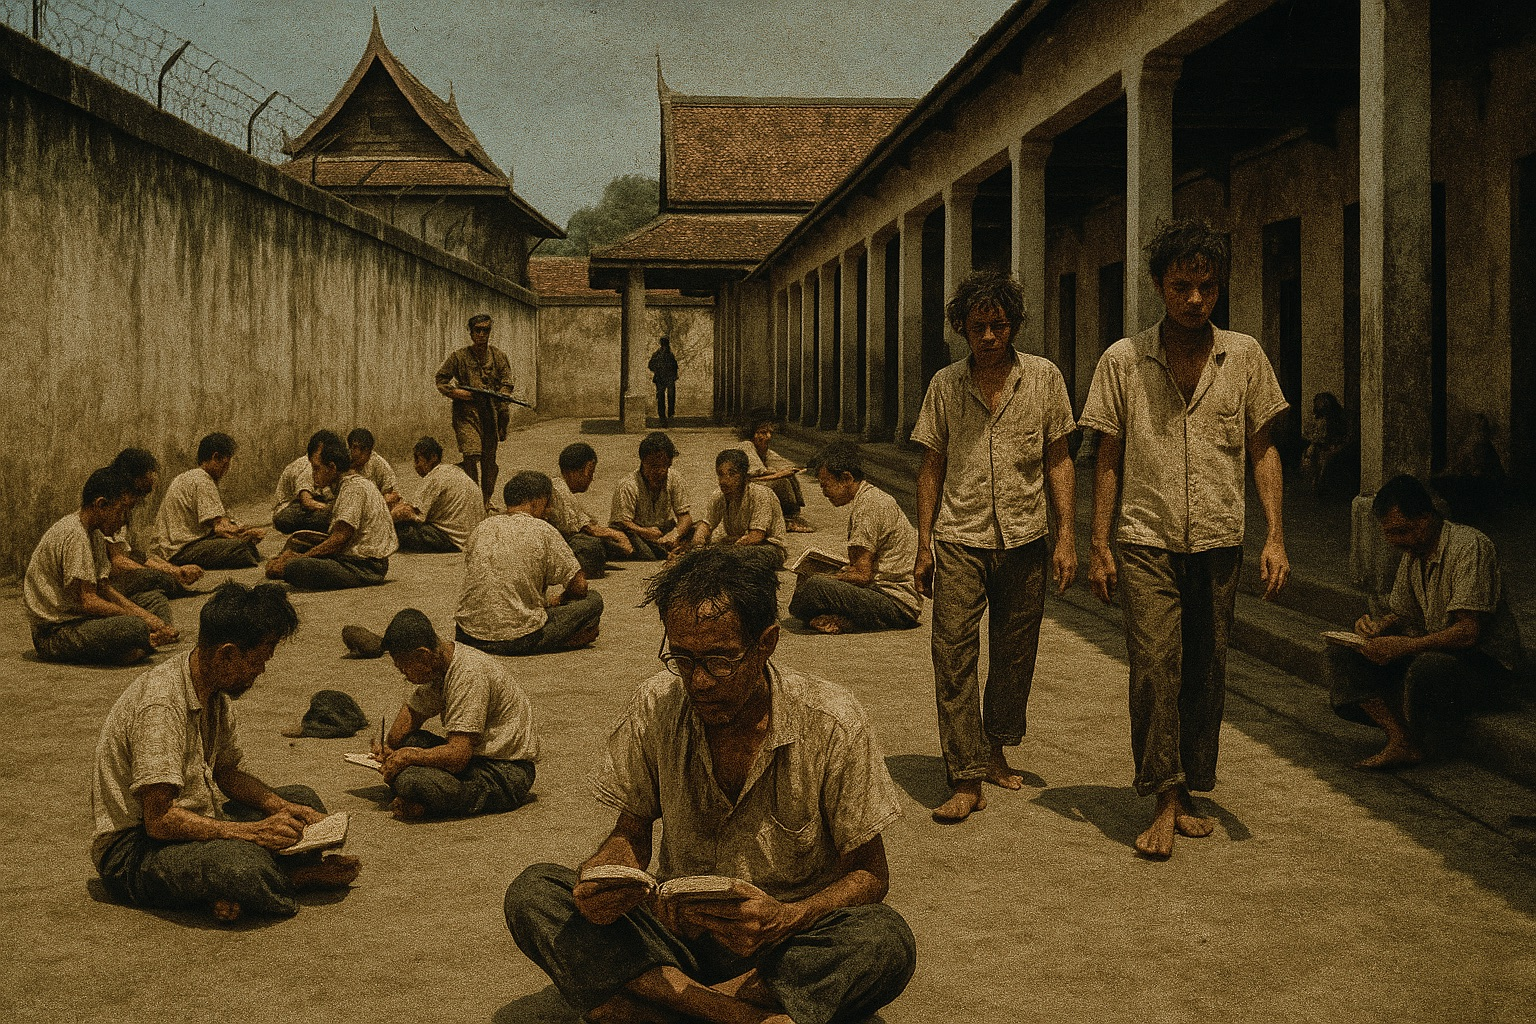
\includegraphics[keepaspectratio]{../_resources/assets/images/ch5-BangKwang.jpeg}}

}

\caption{Bang Kwang prison, surrounded by high concrete walls and
electrified razor wire, where political prisoners from 1933 transformed
Ward Six into an unlikely center of learning and cultural exchange.}

\end{figure}%

The irony was almost too bitter to contemplate. The men whom the
revolutionary government had imprisoned as enemies of progress would
create, within the confines of Bang Kwang prison, one of the most
remarkable educational experiments in Thai history. The political
prisoners whose ``reactionary'' ideas had supposedly made them unfit for
participation in the new Thailand would demonstrate, through their
response to confinement, an intellectual vitality and commitment to
learning that surpassed anything achieved by their captors.

When So Sethaputra arrived at Bang Kwang in early 1934, following his
conviction for sedition (as described in
Chapter~\ref{sec-coup-aftermath}), he entered a world that defied every
expectation about prison life. The forbidding concrete walls topped with
electrified razor wire enclosed not the brutalized, demoralized
population one might expect, but rather a community of scholars,
teachers, and students who had transformed their cells into classrooms
and their shared imprisonment into an opportunity for unprecedented
cultural exchange.

\section{The Architecture of
Confinement}\label{the-architecture-of-confinement}

Bang Kwang prison had been built in 1931 as a modern, high-security
facility designed to house common criminals according to the latest
penological theories. The prison's design reflected contemporary ideas
about criminal rehabilitation: individual cells to prevent the
contamination of minor offenders by hardened criminals, open corridors
to facilitate surveillance, and workshops where prisoners could learn
useful trades. What the designers had not anticipated was that Ward Six
would be filled not with ordinary criminals but with some of the most
educated and accomplished men in Thailand.

Ward Six had been hastily redesigned after the 1932 coup to accommodate
the influx of political prisoners. Each chamber was widened to house
twelve men in what had originally been designed as single-occupancy
cells. The overcrowding was severe, but it had an unexpected benefit: it
forced the prisoners into close contact with one another, creating
opportunities for intellectual exchange that would not have existed in a
conventional prison setting.

The fifty chambers of Ward Six housed a remarkable cross-section of the
old elite: former cabinet ministers and senior civil servants, military
officers who had remained loyal to the monarchy, university professors
and journalists, lawyers and engineers, even members of the royal
family. Many possessed advanced degrees from European and American
universities. Their collective expertise spanned virtually every field
of human knowledge, from agriculture and medicine to literature and
philosophy.

The open corridor that connected all the chambers became the main
thoroughfare of an impromptu university campus. Prisoners would gather
in small groups to discuss everything from Buddhist philosophy to modern
engineering, from Thai classical literature to contemporary European
politics. The guards, most of whom were poorly educated, found
themselves supervising discussions that were entirely beyond their
comprehension.

\section{The Emergence of an Educational
Community}\label{the-emergence-of-an-educational-community}

The transformation of Ward Six into an educational community began
almost immediately after the arrival of the first political prisoners.
Unlike common criminals, who typically responded to incarceration with
despair or rage, these men possessed both the intellectual resources and
the cultural background necessary to create meaning from their
suffering. They understood imprisonment not merely as punishment but as
an opportunity to pursue activities that their previous busy lives had
prevented.

The initiative came from the most senior prisoners, men like Prince
Sithiporn Kridakorn, brother of Prince Bovoradej and a trained
agronomist who had managed experimental farms before his arrest. Prince
Sithiporn quickly emerged as the spiritual leader of the political
prisoners, a man whose aristocratic bearing and genuine concern for
others made him a natural focal point for communal activities. His
decision to offer classes in agriculture and animal husbandry to younger
prisoners established the precedent that others would follow.

The educational system that emerged was entirely informal but remarkably
systematic. Prisoners with expertise in various fields volunteered to
teach others, while those who lacked formal education but possessed
practical skills contributed their own knowledge to the collective
enterprise. The result was a curriculum more diverse and practical than
that offered by most universities, taught by instructors whose
qualifications were impeccable and whose commitment to their students
was absolute.

The classes served multiple purposes beyond simple education. They
provided structure to days that might otherwise have been filled with
despair and boredom. They maintained the intellectual sharpness of men
who might otherwise have deteriorated mentally during long years of
confinement. Most importantly, they preserved and transmitted cultural
knowledge that the revolutionary government seemed determined to
eliminate from Thai society.

\section{So Sethaputra's English
Classes}\label{so-sethaputras-english-classes}

So's decision to offer English-language reading and writing classes
reflected both his personal expertise and his recognition of his fellow
prisoners' needs. His years as Royal Spokesman had made him fluent in
English not merely as a technical language but as a medium of cultural
expression. His extensive knowledge of English literature, combined with
his understanding of Thai educational needs, made him uniquely qualified
to serve as a bridge between Eastern and Western intellectual
traditions.

Cell 42, where So conducted his classes, became one of the most popular
destinations in Ward Six. Former students would later recall the scene:
``Professor Sor Sethaputra, small and frail, with huge eyeglasses that
framed his face, sat cross-legged, propped up by a folded mattress
against the wall, his students forming a half circle around him.'' The
intimate setting created an atmosphere of intense intellectual
engagement that would have been impossible in a conventional classroom.

So's teaching method reflected his deep understanding of Thai learning
styles and his appreciation for the challenges faced by Thai students of
English. Rather than focusing on grammar rules or vocabulary lists, he
emphasized reading comprehension and cultural understanding. He ordered
non-political books and magazines from outside sources, borrowed
materials from the Neilson Hays Library in Bangkok, and gradually built
up a substantial collection of English-language materials within the
prison.

The curriculum So developed was far more sophisticated than anything
available in Thai schools of the period. Students progressed from simple
texts to complex works of literature, from basic conversation to
advanced composition. So's background in journalism proved invaluable,
as he was able to teach not only the mechanics of English but also the
art of clear, persuasive writing. Many of his students would later
credit their prison English classes with providing them with skills that
proved invaluable in their post-prison careers.

\section{The Broader Educational
Ecosystem}\label{the-broader-educational-ecosystem}

So's English classes were just one component of a remarkably diverse
educational program that emerged within Ward Six. The range of subjects
offered reflected the varied backgrounds of the political prisoners and
their commitment to sharing knowledge across disciplinary boundaries.
The result was an interdisciplinary approach to education that was
decades ahead of its time.

Phraya Saraphai Phipat, a naval captain who had served in the royal navy
before his arrest, chose to study rather than teach, enrolling in
Mandarin classes offered by a Chinese prisoner suspected of communist
sympathies. His decision to learn from a fellow prisoner rather than
assert his own expertise demonstrated the egalitarian spirit that
characterized the Ward Six educational community. Rank and social
position, while not entirely forgotten, became less important than
knowledge and teaching ability.

Other senior prisoners offered instruction in their areas of expertise.
Lawyers conducted seminars on legal theory and constitutional law, using
their enforced leisure to explore theoretical questions they had never
had time to consider during their active careers. Engineers explained
principles of construction and design to students who had never
previously shown interest in technical subjects. Medical doctors
provided basic health education to prisoners whose backgrounds had given
them little understanding of hygiene and disease prevention.

The most remarkable aspect of the educational program was its voluntary
nature. No prisoner was required to attend classes, and no formal
credentials were offered. Students participated purely out of
intellectual curiosity and desire for self-improvement. Teachers
volunteered their time and expertise without compensation, motivated
solely by the satisfaction of sharing knowledge and maintaining
intellectual activity during their confinement.

\section{The Discovery of a Mission}\label{the-discovery-of-a-mission}

It was in this environment of intense intellectual exchange that So made
the discovery that would define the remainder of his life. His English
students, despite their intelligence and motivation, consistently
struggled with the same problem: they could read English texts with
reasonable accuracy, but they understood very little of what they read.
The gap between technical reading ability and genuine comprehension was
enormous and frustrating for both students and teacher.

The realization that his students ``clearly needed a good dictionary''
was the genesis of what So would call his ``Life's Work.'' The first
comprehensive English-Thai dictionary written by a Thai for Thai
students was conceived not in a university or research institute but in
a prison cell, born of one man's recognition of his students' needs and
his own capacity to meet them. The project that would consume the next
eleven years of his life began as a simple response to a pedagogical
problem.

So's decision to undertake such an ambitious project while serving a
life sentence might seem irrational, even delusional. But it reflected
both his character and his circumstances. At thirty, he was still
intellectually vigorous and psychologically resilient. His confinement,
while physically restricting, had freed him from the distractions and
obligations that had previously limited his scholarly work. Most
importantly, his teaching experience had given him a clear understanding
of exactly what kind of dictionary Thai students needed.

The project also provided So with something essential for psychological
survival: a sense of purpose that transcended his immediate
circumstances. Rather than viewing his imprisonment as the end of his
useful life, he could see it as an opportunity to make a contribution to
Thai education that would outlast both his captors and himself. The
dictionary would be his revenge against the revolutionaries who had
destroyed his political career---not through violence or political
resistance, but through intellectual achievement that would benefit
future generations of Thai students.

\section{The Transformation of Ward
Six}\label{the-transformation-of-ward-six}

As So began the preliminary work on his dictionary project, the entire
atmosphere of Ward Six was transformed by the educational activities
taking place within its walls. What had been designed as a place of
punishment and isolation became a center of learning and cultural
preservation. The political prisoners, rather than being crushed by
their confinement, had created an intellectual community that rivaled
the best academic institutions in Thailand.

The daily routine in Ward Six came to resemble that of a residential
college more than a prison. Prisoners would rise early and spend the
morning hours in various classes or study groups. Afternoons might be
devoted to individual research or writing projects, while evenings were
often occupied with discussions that continued late into the night. The
guards, initially suspicious of any organized prisoner activity,
gradually came to tolerate and even appreciate the civilized atmosphere
that the educational program created.

The success of the Ward Six experiment attracted attention from other
parts of the prison. Common criminals, initially hostile to the
political prisoners whom they viewed as privileged, began to request
admission to various classes. The educational program thus became a
bridge between different categories of prisoners, breaking down barriers
that might otherwise have led to conflict and violence.

More importantly, the intellectual vitality of Ward Six began to
influence the broader Thai cultural landscape. Books and articles
written by political prisoners were smuggled out of the prison and
circulated among sympathetic intellectuals on the outside. The ideas
developed in prison discussions found their way into underground
political movements and reform organizations. The government's attempt
to silence the old elite had inadvertently created a center of
intellectual resistance that was more influential than the prisoners'
previous political activities had ever been.

As we shall see in Chapter~\ref{sec-dictionary-begins}, So's dictionary
project would become the most ambitious and successful of the many
educational initiatives that emerged from Ward Six. But it was the
collaborative, intellectually stimulating environment of the prison
university that made such an achievement possible. The men whom the
revolution had branded as enemies of progress had created, in their
confinement, a model of educational excellence that would inspire Thai
intellectuals for generations to come.

\bookmarksetup{startatroot}

\chapter{The Dictionary Project Begins}\label{sec-dictionary-begins}

\section{``How Does One Write a Dictionary in
Prison?''}\label{how-does-one-write-a-dictionary-in-prison}

Faced with a life sentence and his students' need for English
translation, So Sethaputra embarked on what he called his ``Life's
Work'' - creating Thailand's first comprehensive English-Thai dictionary
written by a Thai for Thai students.

\begin{figure}[H]

{\centering \pandocbounded{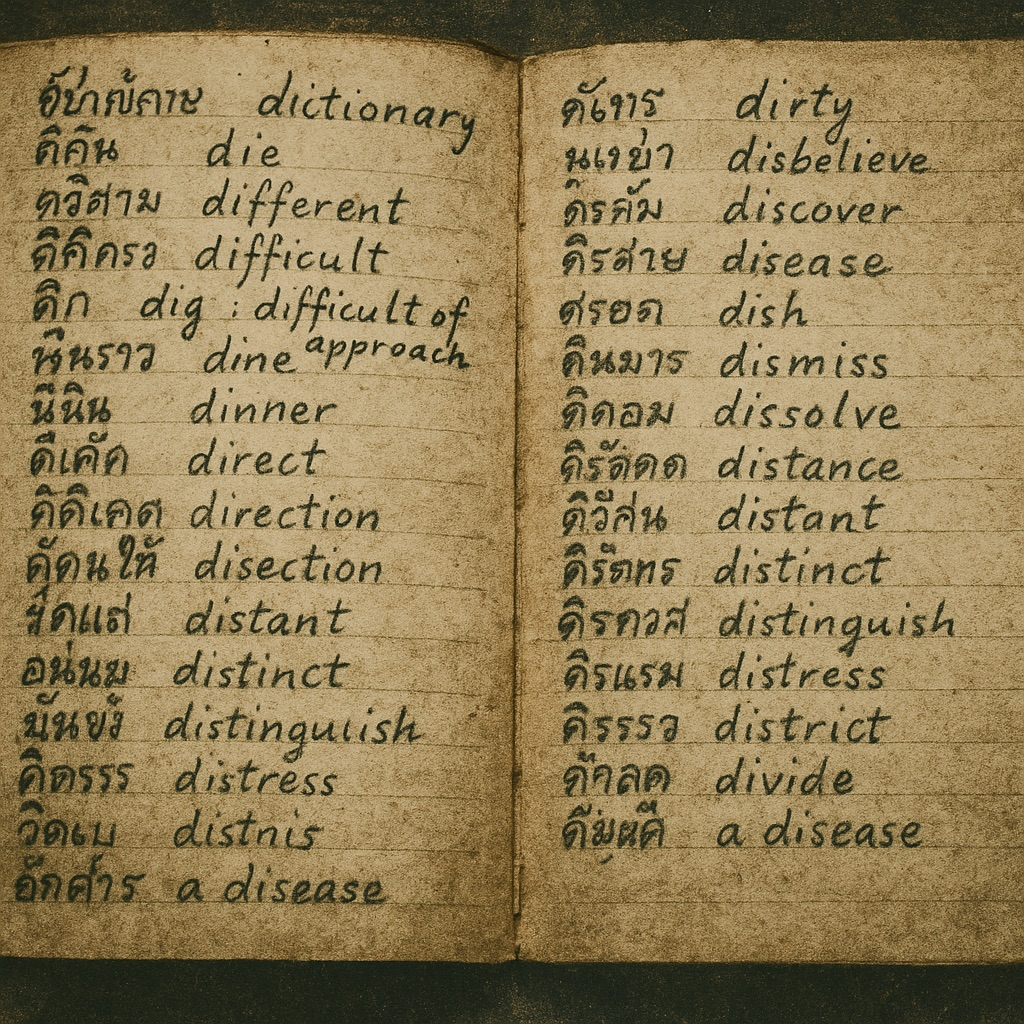
\includegraphics[keepaspectratio]{../_resources/assets/images/ch6-dictionarysample.jpeg}}

}

\caption{A sample page from So Sethaputra's ``New Model English-Siamese
Dictionary,'' showing his innovative approach of using vivid example
sentences drawn from current affairs, personal experience, and Thai
cultural context to illuminate English word meanings for Thai students.}

\end{figure}%

The question that kept So Sethaputra awake during his first weeks in
Bang Kwang prison was deceptively simple yet overwhelmingly complex:
``How does one even begin to write a dictionary in prison?'' The more he
contemplated the practical challenges involved, the more impossible the
task seemed. Yet it was precisely this impossibility that made the
project so compelling. If he could succeed in creating a comprehensive
English-Thai dictionary under such circumstances, he would demonstrate
that intellectual achievement could transcend any form of political
persecution.

The inspiration for the dictionary had emerged from his teaching
experience in Ward Six (as described in
Chapter~\ref{sec-prison-university}), but the decision to undertake such
an ambitious project required a fundamental reorientation of how So
understood his imprisonment. Rather than viewing his life sentence as
the end of his productive career, he began to see it as an unprecedented
opportunity to focus entirely on scholarly work without the distractions
and obligations that had previously limited his intellectual pursuits.

At thirty years old, So possessed the intellectual vigor and
psychological resilience necessary for such a demanding undertaking. His
years as Royal Spokesman had given him extensive experience with both
English and Thai, while his background in journalism had taught him the
importance of clear, accessible prose. Most crucially, his teaching
experience had shown him exactly what kind of dictionary Thai students
needed: not merely a collection of word equivalents, but a comprehensive
guide to English language and culture written from a Thai perspective.

\section{The Vision of a New Kind of
Dictionary}\label{the-vision-of-a-new-kind-of-dictionary}

So's conception of his dictionary project was revolutionary in its scope
and approach. Existing English-Thai dictionaries were typically crude
compilations produced by European scholars or missionaries who lacked
deep understanding of Thai culture and learning styles. These works
treated language as a mechanical process of word substitution, ignoring
the cultural contexts that gave words their real meaning and
significance.

So envisioned something entirely different: a dictionary that would
serve as a bridge between civilizations rather than merely a tool for
translation. Each English word would be explained not through dry
definitions but through vivid example sentences that illuminated both
the word's meaning and its cultural significance. The dictionary would
teach Thai students not just how to translate English words but how to
understand the English-speaking world itself.

The sample page that survives from So's work demonstrates his innovative
approach. Rather than providing abstract definitions, he created example
sentences that were simultaneously educational and culturally relevant.
When defining ``abdicate,'' he wrote simply: ``His Majesty abdicated.''
For ``absent,'' he chose: ``Freedom of the press is absent.'' The entry
for ``accuse'' read: ``They were accused of treason.'' Each example was
drawn from So's own experience and reflected the political realities
that had shaped his life.

This approach required not just linguistic expertise but profound
cultural understanding. So had to comprehend not only what English words
meant but how they functioned within English-speaking societies, then
find ways to convey that understanding to Thai readers who might never
leave their homeland. The dictionary thus became a work of cultural
translation as much as linguistic scholarship.

\section{The Practical Challenges of Secret
Scholarship}\label{the-practical-challenges-of-secret-scholarship}

The practical obstacles facing So's dictionary project seemed almost
insurmountable. Prison regulations strictly forbade political prisoners
from writing anything intended for outside readership beyond personal
letters. All correspondence was carefully censored, and any manuscripts
discovered by guards would be confiscated and their authors punished.
The fundamental problem was not merely writing in secret but finding
ways to preserve and transmit the completed work.

So's solution demonstrated the ingenuity that would characterize his
entire approach to the project. He would disguise his dictionary work as
part of his English teaching activities in Ward Six. The guards, most of
whom were poorly educated and spoke no English, could not distinguish
between legitimate classroom materials and dictionary manuscripts. So's
reputation as a dedicated teacher provided perfect cover for his
scholarly activities.

The physical challenges were equally daunting. So needed writing
materials, reference books, and workspace suitable for sustained
intellectual effort. He solved these problems through a combination of
resourcefulness and careful negotiation. Writing paper and instruments
could be obtained through arrangements with guards who were willing to
supplement their meager salaries through small commercial transactions.
Reference materials could be borrowed from the Neilson Hays Library or
purchased from outside sources under the pretense of supporting his
English classes.

Most ingeniously, So designed and constructed a functional writing desk
and comfortable chair from packing crates available within the prison.
This improvised furniture provided him with a proper workspace that was
essential for the meticulous work of dictionary compilation. The
psychological importance of having a dedicated study area cannot be
overstated; it created a sense of scholarly normalcy that helped
maintain his intellectual focus despite the abnormal circumstances of
his confinement.

\section{The Recruitment of
Collaborators}\label{the-recruitment-of-collaborators}

The scope of the dictionary project required assistance that So could
not provide alone. Fortunately, Ward Six contained numerous educated
prisoners who were eager to contribute to meaningful intellectual work.
So's organizational skills and natural leadership abilities enabled him
to create an efficient collaborative system that maximized the talents
of his fellow inmates while maintaining the secrecy necessary for the
project's survival.

So instituted a strict daily routine that provided structure for both
his own work and that of his assistants. The team would begin work at
seven-thirty in the morning and continue until lunch break at
eleven-thirty, then resume at two-thirty in the afternoon and work until
dark. This schedule provided approximately eight hours of productive
work time each day, far more than So could have achieved working alone.

The division of labor was carefully planned to utilize each assistant's
particular strengths. Some prisoners excelled at the meticulous physical
transcription required to produce clean copies of So's drafts. Others
had beautiful handwriting that was essential for preparing the final
manuscript versions. Still others possessed specialized knowledge that
could inform particular dictionary entries. The result was a
collaborative scholarly enterprise that demonstrated the intellectual
vitality of the imprisoned elite.

So's role in this system was that of the creative brain while his
assistants provided the skilled labor necessary to transform his ideas
into finished products. Former collaborators would later recall the
magical moments when ``Sor was the brain and we were the labour. He
would sit there, cross-legged, and suddenly burst out with a word or
phrase; and we would immediately transcribe it onto paper.'' This method
allowed So to maintain the creative flow essential for productive
scholarship while ensuring that his ideas were immediately captured and
preserved.

\section{The Critical Role of
Gaysorn}\label{the-critical-role-of-gaysorn}

The most dangerous aspect of the entire enterprise was smuggling
completed manuscript pages out of the prison past the security
checkpoints that separated Ward Six from the outside world. This
seemingly impossible task was accomplished through the heroic efforts of
So's mother, Gaysorn, whose devotion to her son's work made the
dictionary project possible.

Gaysorn had remained in Bangkok throughout So's imprisonment, dedicating
her life to supporting his scholarly activities. Her literacy, unusual
for women of her generation, made her uniquely qualified to serve as her
son's collaborator and co-conspirator. She understood not only the
practical importance of the dictionary project but also its deeper
significance as a form of cultural resistance against the revolutionary
government that had destroyed her son's political career.

The smuggling operation required remarkable ingenuity and courage.
Gaysorn developed several methods for concealing manuscript pages during
her prison visits. Her primary technique involved using the outer
cylinder of a large thermos flask to hide rolled-up papers. The false
bottom could accommodate several pages at a time, and the device
appeared entirely innocent to guards who were accustomed to visitors
bringing food and beverages to prisoners.

When the thermos flask method became risky due to repeated use, Gaysorn
introduced a false-bottomed basket that could conceal even more
material. So must have appreciated the irony when he later wrote the
dictionary entry: ``false: The documents were concealed under the false
bottom of the box.'' His mother's smuggling activities had provided him
with perfect real-world examples for his scholarly work.

Over the course of several years, Gaysorn successfully smuggled almost
2,000 pages of manuscript material out of Bang Kwang prison. This
represented not merely a logistical achievement but a act of remarkable
courage. Discovery would have meant severe punishment for both mother
and son, and the complete destruction of years of scholarly work. Her
success made possible everything that followed in So's dictionary
project.

\section{The Publishing Innovation}\label{the-publishing-innovation}

By the time So had completed work through the letter ``G,'' he felt
confident enough in the project's quality and his mother's smuggling
abilities to begin considering publication arrangements. This decision
required him to move from purely scholarly concerns to practical
questions of marketing and distribution. The challenge was to find a
publisher willing to handle material produced by a political prisoner
and to develop a distribution system that would not compromise the
secrecy essential to the project's continuation.

So's solution was to contact Phraya Nibhon Pojanart, owner of Krungdheb
Bannakarn, Bangkok's leading bookstore. Phraya Nibhon was a member of
the old elite who had avoided imprisonment but remained sympathetic to
the political prisoners' plight. More importantly, he possessed the
commercial expertise and distribution network necessary to bring So's
dictionary to market.

The publishing arrangement that So and Phraya Nibhon developed was
brilliant in both its commercial and political aspects. Rather than
attempting to publish the complete dictionary at once, which would have
required enormous capital investment and created dangerous exposure for
all involved, they decided to issue the work in weekly installments over
a period of two years. Subscribers could collect the installments and
bind them into two volumes totaling 2,400 pages when the series was
complete.

This serialization approach solved multiple problems simultaneously. It
required minimal upfront investment from the publisher, reducing
financial risk and making the project commercially viable. It provided
So with regular income throughout his imprisonment, addressing the
economic hardship that affected his family. Most importantly, it created
plausible deniability for the political aspects of the project.

The official line developed by Phraya Nibhon was that he had
commissioned the dictionary from So between 1927 and 1932, well before
his imprisonment for political activities. This fiction allowed both
publisher and author to avoid charges of conducting illegal business
with a political prisoner. The completed portions of the dictionary
could be presented as legitimate commercial inventory rather than
contraband material produced in violation of prison regulations.

\section{The Market Response}\label{the-market-response}

The first installments of ``The New Model English-Siamese Dictionary''
exceeded all expectations for commercial success. Thai students and
intellectuals, starved for high-quality educational materials, embraced
So's work with enthusiasm that surprised even its creators. The
dictionary was unlike anything previously available in Thailand, and its
innovative approach to English-language instruction filled a crucial gap
in the country's educational resources.

The success owed much to So's deep understanding of his target audience.
Unlike European-produced dictionaries that assumed readers possessed
extensive cultural knowledge of the English-speaking world, So's work
was designed specifically for Thai students who were encountering
English language and culture for the first time. His example sentences
drew on Thai historical experiences, contemporary political events, and
cultural references that would be immediately meaningful to his readers.

The commercial success of the early installments provided So with
something almost as valuable as income: validation that his years of
work were producing something of genuine value to Thai society. The
positive market response demonstrated that his scholarly activities were
not merely personal therapy or intellectual self-indulgence, but rather
a significant contribution to his country's educational development.

The regular income from dictionary sales also addressed a crucial
practical problem. So was supporting not only himself but also his
younger brother and sister, who were attending university. The
revolutionary government's destruction of his political career had
eliminated his family's primary source of income, making the dictionary
earnings essential for their economic survival. The project thus served
both scholarly and practical purposes, demonstrating how intellectual
achievement could provide concrete benefits even under the most
difficult circumstances.

As we shall see in Chapter~\ref{sec-rising-storm}, So's dictionary work
would continue to evolve and expand even as the broader political
situation in Asia deteriorated. The global crisis that would eventually
engulf Thailand in world war would create new challenges for the
dictionary project, but it would also demonstrate the remarkable
resilience of intellectual endeavor in the face of political upheaval.
So's ``Life's Work'' had begun as a response to his students' needs, but
it would ultimately become a testament to the power of scholarship to
transcend the limitations imposed by political persecution.

\bookmarksetup{startatroot}

\chapter{Rising Storm}\label{sec-rising-storm}

\section{Japan's Shadow Over Southeast
Asia}\label{japans-shadow-over-southeast-asia}

As So continued his dictionary work in prison, the storm clouds of war
gathered across Asia, with Japan's expanding empire casting an
increasingly dark shadow over Thailand and the entire region.

While So Sethaputra worked methodically through the alphabet in his
prison cell (as described in Chapter~\ref{sec-dictionary-begins}),
forces beyond Thailand's borders were reshaping the global order in ways
that would ultimately reach even into the remote chambers of Bang Kwang
prison. The dictionary project that had begun as a response to his
students' educational needs was proceeding in a world increasingly
dominated by military conflict and imperial ambition. The same
international tensions that had influenced Thailand's internal political
transformation were now building toward a global conflagration that
would test every nation's capacity for survival.

The Japan that cast its expanding shadow over Southeast Asia in the late
1930s was a nation transformed by its own revolutionary upheaval. Just
as Thailand had experienced the trauma of political transformation in
1932, Japan had undergone its own internal convulsions as military
leaders gained ascendancy over civilian politicians. The parallels were
not lost on thoughtful observers: both countries had seen traditional
elites displaced by new forms of authoritarianism, both had witnessed
the triumph of military values over civilian expertise, and both were
now governed by men who believed that force could solve problems that
diplomacy had failed to address.

\section{The Imperial Vision}\label{the-imperial-vision}

Japan's vision for Asia was as comprehensive as it was ambitious. The
concept of the Greater East Asia Co-Prosperity Sphere promised to
liberate Asian peoples from European colonial domination while
establishing Japan as the region's natural leader. This ideology
appealed to anti-colonial sentiment throughout Asia, including among
some Thai intellectuals who saw Japan as proof that Asian nations could
successfully modernize and compete with Western powers.

The appeal of Japanese success was particularly strong among Thai
military officers, who had studied Japanese military reforms and admired
the speed with which Japan had transformed itself from a feudal society
into a modern industrial power. The Japanese victory over Russia in 1905
had demonstrated that Asian nations could defeat European armies, while
Japan's rapid industrialization showed that modernization did not
require abandoning cultural identity. For Thai nationalists seeking
models for their own country's development, Japan offered an attractive
alternative to European patterns of modernization.

However, Japan's vision of Asian liberation came with costs that became
increasingly apparent as the 1930s progressed. Japanese ``liberation''
meant Japanese domination, and Japanese leadership required the
subordination of other Asian nations to Japanese interests. The
Co-Prosperity Sphere was less a partnership of equals than an empire
disguised by anti-colonial rhetoric. This reality became clear as
Japan's military expansion accelerated and its demands on neighboring
countries became more insistent.

The Japanese invasion of Manchuria in 1931, followed by full-scale war
with China beginning in 1937, revealed the true nature of Japanese
intentions. The brutality of Japanese military operations in China
shocked international opinion and demonstrated that Japanese promises of
Asian liberation masked traditional imperial ambitions. For Thailand,
geographically positioned between Japanese-occupied territories and
European colonies, Japan's expansion created both opportunities and
existential threats.

\section{Thailand's Precarious
Position}\label{thailands-precarious-position}

Thailand's geographical location made neutrality increasingly difficult
as Japanese power expanded throughout Southeast Asia. The kingdom found
itself caught between competing imperial powers, each demanding
accommodation while threatening retaliation for insufficient
cooperation. British and French colonial authorities expected Thailand
to support their resistance to Japanese expansion, while Japanese
diplomats made increasingly explicit demands for Thai cooperation with
their regional objectives.

The Thai government that faced these pressures was itself the product of
revolutionary change and remained insecure in its authority. The
military leaders who had overthrown the absolute monarchy in 1932
understood force better than diplomacy, and they were more impressed by
Japanese military success than by European promises of protection. The
destruction of the old diplomatic elite (men like So Sethaputra who had
expertise in international relations) had deprived Thailand of precisely
the kind of sophisticated analysis that the current crisis required.

Thailand's military government was particularly vulnerable to Japanese
pressure because it shared certain ideological affinities with Japanese
authoritarianism. Both regimes had come to power through military coups
that displaced traditional elites, both emphasized nationalism and
modernization, and both viewed parliamentary democracy as an obstacle to
effective governance. These similarities made cooperation with Japan
seem natural, even inevitable, to Thai leaders who saw their own
revolutionary transformation reflected in Japanese political
development.

The economic dimension of Thailand's dilemma was equally compelling.
Japan offered Thailand expanded markets for its agricultural exports and
investment in industrial development that could reduce the kingdom's
dependence on European colonial powers. Japanese economic proposals were
often more generous than European alternatives, and they came without
the political conditions that European powers typically imposed. For a
government seeking to demonstrate its independence and effectiveness,
Japanese partnership offered tangible benefits that were difficult to
ignore.

\section{The Transformation of Regional
Power}\label{the-transformation-of-regional-power}

The collapse of European power in Asia proceeded with startling speed
once Japanese military expansion began in earnest. The fall of Singapore
in February 1942 would mark the definitive end of European colonial
dominance in Southeast Asia, but the erosion of European authority was
already apparent years earlier. French authority in Indochina was
weakened by political instability in France itself, while British power
was increasingly focused on the growing threat from Nazi Germany.

This power vacuum created opportunities for Thailand to reclaim
territories that had been lost to European colonial expansion in
previous decades. The prospect of recovering the Lao territories on the
left bank of the Mekong River and the Cambodian provinces of Battambang
and Siem Reap was enormously appealing to Thai nationalists who had
never accepted these losses as permanent. Japanese support for Thai
territorial claims offered the possibility of reversing decades of
humiliation at European hands.

The Franco-Thai War of 1940-1941 demonstrated both the opportunities and
dangers of Thailand's new international position. Thai military forces,
equipped with modern weapons and supported by Japanese diplomatic
pressure, successfully recovered the desired territories from French
Indochina. However, the victory came at the cost of increased dependence
on Japan, which had mediated the conflict and guaranteed the territorial
settlement. Thailand had gained territory but lost strategic autonomy.

The success of Thai military operations also vindicated the
revolutionary government's emphasis on military modernization and
nationalist ideology. The territorial gains achieved through force
validated the military leadership's approach to governance and
strengthened their position against remaining opposition. The war
demonstrated that the new Thailand could successfully challenge European
power when supported by Asian allies, providing powerful validation for
the anti-European sentiment that had motivated the 1932 revolution.

\section{The Impact on Prison Life}\label{the-impact-on-prison-life}

The changing international situation had immediate consequences for the
political prisoners confined in Bang Kwang prison. As tensions with
European powers increased and cooperation with Japan deepened, the
government became increasingly paranoid about potential fifth-column
activities and foreign espionage. The political prisoners, with their
European educations and international connections, were viewed with
growing suspicion as potential security threats.

Security measures within Bang Kwang were progressively tightened as the
international situation deteriorated. The relatively liberal policies
that had allowed prisoners limited freedom of movement and communication
with the outside world were replaced by stricter controls and more
intensive surveillance. The guards received instructions to conduct more
thorough searches of both prisoners and their correspondence, making it
increasingly difficult to maintain the dictionary project's essential
secrecy.

The economic pressures created by military mobilization and
international tensions also affected prison conditions. Resources that
had previously been available for prisoner welfare were redirected to
military purposes, leading to reduced food rations and deteriorating
living conditions. The guards themselves became more hostile as
nationalist propaganda portrayed the political prisoners as traitors who
had opposed Thailand's national awakening and continued to threaten the
country's security.

Most ominously for So and his fellow prisoners, the government began to
view their proximity to Bangkok as a security liability. The capital's
strategic importance made the presence of potentially disloyal elements
nearby increasingly unacceptable to military planners who were preparing
for possible conflict. The political prisoners' intellectual
capabilities, which had once made them valuable potential contributors
to national development, were now seen as threats to internal security
that required more remote containment.

\section{The Decision to Transfer}\label{the-decision-to-transfer}

The government's decision to transfer the political prisoners from Bang
Kwang to a more remote location reflected both security concerns and the
broader transformation of Thai society under military rule. The
prisoners' European educations and international perspectives, once
valued as assets for national modernization, were now viewed as evidence
of insufficient loyalty to the Thai nation. Their continued presence in
Bangkok represented an unacceptable risk in an increasingly militarized
society.

The choice of Tarutao Island as the new prison location was carefully
calculated to address multiple government concerns. The island's
remoteness would eliminate any possibility of the prisoners influencing
political developments in Bangkok, while its isolation would prevent any
potential rescue attempts by foreign agents. The dangerous waters
surrounding the island would make escape virtually impossible, ensuring
that the prisoners would remain securely contained regardless of how
international conditions might change.

The transfer decision also reflected the government's growing confidence
in its ability to act without regard for international opinion. The
movement of political prisoners to a remote island would undoubtedly
attract criticism from European governments and human rights
organizations, but Thailand's leaders no longer felt compelled to
accommodate such concerns. Japanese support had reduced Thailand's
dependence on European approval, freeing the government to pursue
policies that would have been politically impossible under the old
international system.

For So personally, the transfer represented a devastating blow to the
dictionary project that had become his life's work. The smuggling
operation that his mother had developed with such ingenuity and courage
would become much more difficult to maintain over the greater distances
involved in reaching Tarutao. The reference materials and outside
support that had been essential to the project's success would be much
harder to obtain in such a remote location.

\section{The Broader Pattern of
Militarization}\label{the-broader-pattern-of-militarization}

Thailand's transformation in response to Japanese expansion was part of
a broader pattern of militarization that was reshaping societies
throughout Asia. The traditional emphasis on civilian governance,
diplomatic solutions, and international cooperation was giving way to
military values that prioritized force, hierarchy, and national
self-reliance. The intellectual elite that had once provided leadership
for Asian societies found themselves marginalized by military officers
who viewed intellectual complexity as weakness and international
sophistication as disloyalty.

This transformation had particular significance for men like So
Sethaputra, whose careers had been built on the assumption that
education, expertise, and cultural sophistication would be valued by
modern Asian societies. The rise of military authoritarianism throughout
the region represented not merely a political change but a fundamental
alteration in the criteria by which individuals and ideas were judged.
The qualities that had made the Western-educated elite valuable under
the old system now made them suspect under the new order.

The militarization of Thai society also reflected deeper anxieties about
national identity and cultural authenticity that had been intensified by
the international crisis. The pressure to choose sides in the emerging
global conflict forced Thai leaders to define more clearly what they
meant by Thai nationalism and how Thailand should relate to the
competing forces reshaping the international system. The political
prisoners, with their complex loyalties and international perspectives,
represented an uncomfortable reminder of the ambiguities that the
government preferred to ignore.

As we shall see in Chapter~\ref{sec-tarutao-exile}, the transfer to
Tarutao Island would test both So's personal resilience and the
sustainability of his dictionary project under even more challenging
circumstances. The island that would become their new prison was
beautiful but forbidding, isolated but not empty of dangers. The
political prisoners who had transformed Bang Kwang into an unlikely
center of learning would face the challenge of maintaining their
intellectual community under conditions that were designed to break
their spirit and destroy their capacity for organized resistance.

\bookmarksetup{startatroot}

\chapter{Tarutao Exile}\label{sec-tarutao-exile}

\section{Paradise Lost: The Prison
Island}\label{paradise-lost-the-prison-island}

In 1939, So and his fellow political prisoners were transferred to the
remote island of Tarutao, where the brutal beauty of paradise masked the
harsh realities of their continued imprisonment.

The prows of two small steamers thrust through the dark rippling waters
of Talo Udang Bay and laid anchor three hundred meters offshore at
Tarutao island in southern Thailand. The tide was much too low for the
Adang and the Rawi---converted Japanese fishing boats---to land on the
beach. Seventy passengers, all prisoners, waded ashore in complete
darkness, their belongings balanced precariously on their heads as they
moved slowly through the waist-deep water.

Prisoner number 26, thin and weary yet somehow still in good spirits,
was the last to disembark. As So Sethaputra moved carefully through the
water, his main concern was the safety of the heavy cardboard box
balanced on his head. Its contents represented years of work and the
foundation of his future scholarly endeavors: twenty-two tins of State
Express cigarettes, one tattered 1924 edition of the Concise Oxford
Dictionary (minus cover), several English language classics, sixty
exercise books, five pens and seventy-three nibs, six bottles of ink,
three dozen pencils, and most precious of all, a partially completed
manuscript in longhand.

The transfer from Bang Kwang prison (as described in
Chapter~\ref{sec-rising-storm}) had been undertaken with typical
bureaucratic efficiency but little regard for human comfort. The
prisoners had been given minimal notice of their departure, barely
enough time to gather their few possessions and prepare for an uncertain
future. For So, the move represented a catastrophic disruption to the
dictionary project that had become his life's work, but he was
determined to continue his scholarly activities regardless of the
obstacles that lay ahead.

\section{A Paradise Transformed}\label{a-paradise-transformed}

Today, Tarutao is the headquarters of Southeast Asia's largest marine
park, a tropical paradise where forest-clad hills rise seven hundred
meters above the intense blue Andaman Sea. Its jungles, wet with rain,
stretch down to pristine beaches, while craggy limestone cliffs on the
eastern side plunge dramatically into the ocean. Numerous streams and
waterfalls cut through the mountainous interior, and a thick canopy of
rainforest provides secure habitat for wild boar, long-tailed macaques,
hornbills, and mouse deer. In the azure sea, dolphins, sea turtles,
octopus, rays, and angelfish thrive undisturbed among some of the
world's most spectacular coral reefs.

In 1939, however, for the newly arrived political prisoners who had been
transferred from Bangkok, Tarutao was grim and forbidding. They spent
their first night shivering on the beach, huddled uncomfortably together
in an open makeshift lean-to with just a flimsy palm thatch roof to
protect them from wind and rain. Behind them, the jungle and its dark
menacing forest were foreboding. The piercing screams of wild boars and
the eerie shrills of macaws put fear into their hearts. The cold, wet
monsoon wind slapped noisily against the palm thatch, keeping them awake
for most of the night. By dawn, they were too weary to marvel at the
first gentle rays of the rising sun streaking the eastern sky with
shafts of pink and gold.

The prison camp at Talo Udang Bay, located at the southern end of the
island, had been established as a penal colony for political prisoners
in 1937. There was an existing prison camp for hardened criminals and
murderers on the east coast at Talo Wao Bay. These two prison camps were
separated by a twelve-kilometer track built by the common prisoners, and
the two classes of prisoners were kept apart, although some of the less
dangerous inmates were often called upon to work for the political
prisoners.

Tarutao had been chosen for its distance from Bangkok---over 1,000
kilometers---and for its treacherous shark-infested waters. The
southwest monsoon that battered the western shore from May to October
and the northeast monsoon that hit the eastern side from November to
April made travel to and from the mainland difficult and dangerous.
Escape was not an option, or so the authorities believed.

\section{The Moment of Decision}\label{the-moment-of-decision}

So Sethaputra had no intention of escaping, although escape had become
the main topic of discussion among the political prisoners during their
first weeks on the island. So had his own agenda: he had to finish his
life's work. The dictionary project that had consumed years of his
imprisonment at Bang Kwang could not be abandoned simply because of a
change of venue. If anything, the isolation of Tarutao might provide
even better conditions for sustained scholarly work, once the immediate
challenges of establishing a new routine could be overcome.

The dramatic change in living conditions forced immediate decisions
about priorities and survival strategies. The prisoners quickly split
into two distinct groups: those who wanted to escape to Langkawi island
five kilometers south across the sea in Malaya, and those who were too
old, too frightened, or not prepared to take additional risks. The
division reflected not only practical assessments of escape
possibilities but also fundamentally different approaches to their
imprisonment and their responsibilities to family and scholarly
commitments.

So had been part of an original escape committee formed at Bang Kwang,
which included two of his former colleagues at the Daily Mail: Louis
Kiriwat, the editor, and Naval Captain Phraya Saraphai, a contributor.
They had invited many of their close friends from Ward Six to join their
cause, including So's closest friend and confidant, Prince Sithiporn, a
man he respected highly. However, Prince Sithiporn had declined,
asserting that at sixty he was too old and did not want to be a burden
to the group.

After much soul-searching, So also decided not to join the escape group,
even though he had been one of the early planners. His decision was
influenced by multiple factors, each reflecting different aspects of his
character and circumstances. The most immediate influence came from his
mother, Gaysorn, who had communicated to him from Satun on the mainland
where she was staying in order to be near her son. Her message was
simple but compelling: ``Don't go.''

\section{The Wisdom of Restraint}\label{the-wisdom-of-restraint}

Gaysorn's advice reflected her practical wisdom and deep understanding
of both the risks involved in escape and the opportunities that might be
lost if So abandoned his scholarly work. She was concerned for her son's
safety, recognizing that the dangers of escape extended far beyond the
immediate risks of capture or drowning. Even if So successfully reached
Malaya, he would become a political refugee with no means of support and
no way to continue the dictionary project that had become his defining
achievement.

More importantly, Gaysorn understood that a regular income from the
dictionary was the most important priority for the family's survival. So
was the only breadwinner, supporting not only himself but also his
younger brother and sister who were attending university. The
revolutionary government's destruction of his political career had
eliminated the family's primary source of income, making the dictionary
earnings essential for their economic survival.

So also chose to stay in order to complete the unfinished dictionary. He
felt a moral obligation to his publisher, Phraya Nibhon, and to the
subscribers who had supported the project from its beginning. He
understood that if his escape came to the attention of the authorities,
the printing press would certainly be shut down. After all, how could
the government tolerate a book written by a political fugitive being
published, even if it was ``just'' a dictionary?

The commercial success of the early installments had provided So with
several thousand baht in royalties, thanks to his loyal subscribers. He
could never let them down by abandoning the project before its
completion. The dictionary had become more than a personal scholarly
achievement; it was a commitment to Thai education and culture that
transcended his individual circumstances.

\section{The Great Escape}\label{the-great-escape}

\begin{figure}[H]

{\centering \pandocbounded{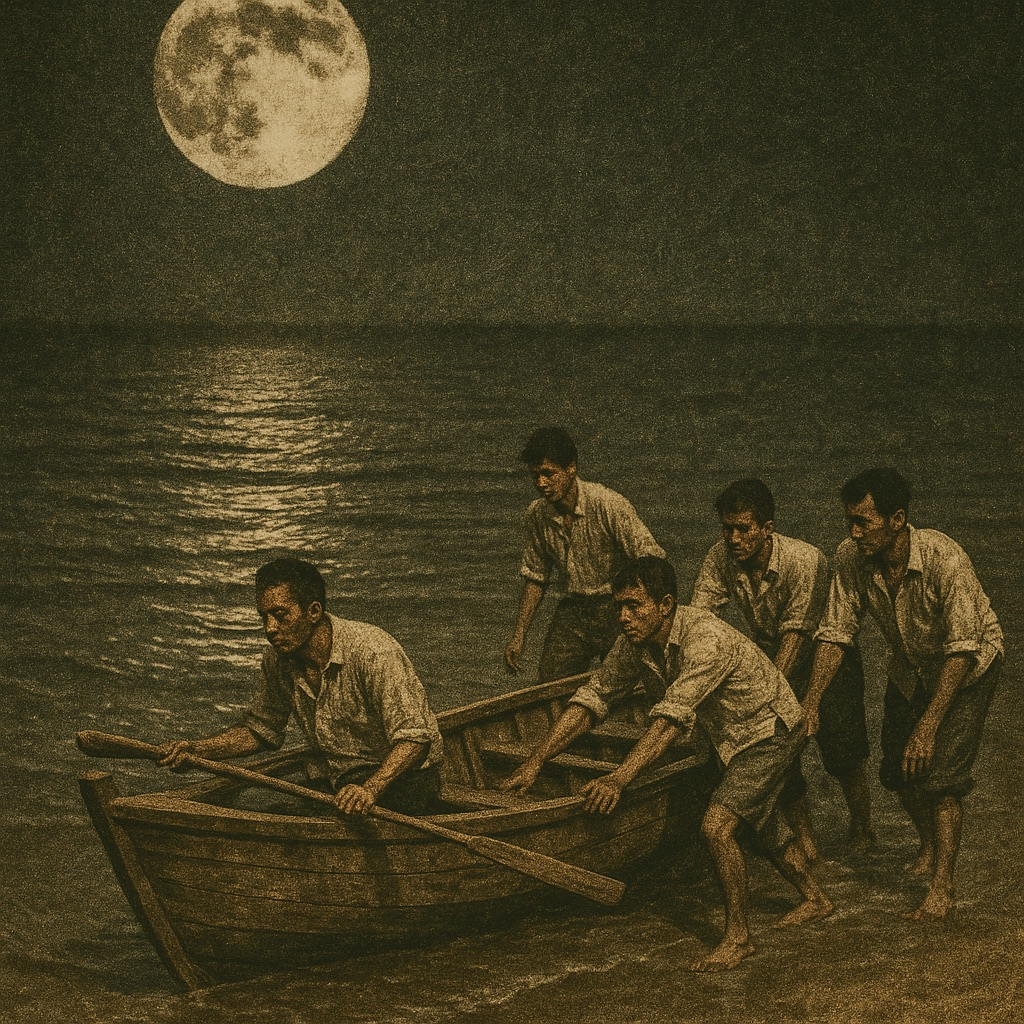
\includegraphics[keepaspectratio]{../_resources/assets/images/ch8-DaringEscape.jpeg}}

}

\caption{Captain Phraya Saraphai and his fellow conspirators prepare for
their daring nighttime escape from Tarutao prison island to Langkawi,
Malaya. The five political prisoners risked shark-infested waters and
monsoon conditions in their desperate bid for freedom on a moonlit night
in 1939.}

\end{figure}%

On a full moon night, day twenty-nine of their stay on Tarutao, five
prisoners decided to make their escape to Langkawi by boat, led by
Captain Phraya Saraphai. The other four were Louis Kiriwat, So's old
colleague from the Daily Mail; Colonel Phraya Suraphan; Chalam
Liamphetchrat, a lawyer who was also a keen astrologer and had selected
the auspicious date for their escape; and Kuhn Asaniratakarn, a railway
engineer.

It was a sad moment for So when they made their farewells on the beach.
They had worked, laughed, and suffered together for so long that their
separation felt like the breaking of family bonds. The men who were
leaving represented some of the finest minds of their generation,
individuals whose expertise and experience would be desperately needed
for Thailand's future development. Their departure diminished not only
the prison community but also the kingdom's intellectual resources.

So's decision to remain was supported by Prince Sithiporn, who told him
that the dictionary would be his gift to future generations. This
perspective helped So understand his choice not as a failure of courage
but as a commitment to cultural preservation that would outlast the
political conflicts that had created their current circumstances. The
dictionary project represented a form of resistance more enduring than
political rebellion: the preservation and transmission of knowledge
across generational and cultural boundaries.

The escape attempt itself was both audacious and carefully planned. The
conspirators had studied the tides, weather patterns, and patrol
schedules for weeks before making their attempt. They had constructed a
makeshift boat from materials available on the island and had gathered
supplies for the dangerous journey across open water. Their departure in
the darkness of early morning was witnessed only by the few prisoners
who had chosen to remain behind.

\section{Building a New Community}\label{building-a-new-community}

Those who had made the decision to remain on the island responded with a
conscious effort to rebuild their lives under the new circumstances.
Over the next few weeks, they set about improving their living
conditions by building new living quarters, decent kitchens, and clean
latrines. Fortunately, fresh water was freely available from the many
streams on the island, providing one essential resource that would not
be a limiting factor in their survival efforts.

Prince Sithiporn put his heart and soul into working the land, making
the earth more arable and eventually producing enough vegetables and
fruit to keep everyone healthy. His agricultural expertise, gained from
managing experimental farms before his imprisonment, proved invaluable
in transforming Tarutao from a place of confinement into a productive
community. The prince became the spiritual leader of the former inmates
of Ward Six, continually boosting their morale and treating So like a
son during this difficult period of adjustment.

The physical transformation of their living environment was accompanied
by a psychological adjustment that required considerable time and
effort. The prisoners had to adapt from the structured routine of Bang
Kwang prison to the more flexible but also more demanding requirements
of semi-self-sufficient living. They had to learn new skills, establish
new social relationships, and find ways to maintain their intellectual
activities under very different circumstances.

It was difficult for So to work on his dictionary under these trying
conditions. He was missing the privileged status he had enjoyed at Bang
Kwang, where his reputation as a teacher and scholar had provided both
protection and resources for his work. He was also pining for Sompong,
his newly wedded wife, whom he had married during one of the brief
periods when political prisoners were allowed outside Bang Kwang for day
visits.

\section{The Resumption of Scholarly
Work}\label{the-resumption-of-scholarly-work}

Since So was not a religious person and did not believe in God, he did
not seek holy guidance in prayer or spiritual meditation like many other
prisoners. Instead, he took solace in his work, and through sheer
determination and strength of character, he was soon able to return to
his ``Life's Work.'' The dictionary project provided him with the
psychological anchor he needed to maintain his sanity and sense of
purpose under the challenging conditions of island imprisonment.

He hired common prisoners to build a separate hut for his workplace and
designed a new desk suitable for the different conditions on Tarutao.
The construction of a dedicated workspace was essential for maintaining
the discipline and focus required for dictionary compilation. The
psychological importance of having a proper study environment cannot be
overstated; it created a sense of scholarly normalcy that helped sustain
his intellectual efforts despite the abnormal circumstances of his
confinement.

So also took special care of his personal hygiene and appearance, never
allowing himself to become demoralized by his circumstances. He was
always well-groomed and made sure that even his threadbare
clothes---white shirt and Chinese silk trousers---remained impeccable
and well-laundered. His hair was always combed, and he arranged for one
of the common prisoners to give him regular haircuts. He understood
instinctively that maintaining his personal standards was essential for
preserving his psychological resilience and his effectiveness as a
scholar and leader.

By June 1940, So reached the letter ``Z'' in his alphabetical
progression through the English language. The giant library edition
dictionary was finished at last, running to 4,000 pages---1,600 more
than originally conceived. The expansion reflected both the thoroughness
of his approach and the additional insights he had gained through years
of sustained work on the project. Now better organized and more mentally
alert than ever, he could start work right away on a desk-sized
dictionary, a smaller version designed specifically for high school
students.

\section{Life in Paradise}\label{life-in-paradise}

In time, So came to prefer life on Tarutao to Bang Kwang. The island was
beautiful, the air was fresh and clean, and the surrounding nature was
peaceful and quiet. Apart from the constant threat of malaria and other
tropical diseases, So and his fellow prisoners led a relatively healthy
life. The natural environment provided a therapeutic setting that was
conducive to both physical and mental well-being, despite the
restrictions of their imprisonment.

Morale improved significantly as the prisoners adapted to their new
circumstances. Everyone chipped in to make prison life as pleasant as
possible, creating a genuine community that was more cohesive and
productive than what they had experienced at Bang Kwang. Prince
Sithiporn, with the help of a group of common prisoners, produced enough
vegetables and fruit for the island's consumption, with surplus marketed
at Satun on the mainland. He also baked bread and cakes in an oven sent
from the mainland by his wife, providing luxuries that would have been
impossible under normal prison conditions.

Not to be outdone, So started to manufacture soap, essential for someone
as particular about personal hygiene as he was. He soon ran out of State
Express cigarettes and started experimenting with different kinds of
leaves, though this was not a huge success. Although So was not a
gourmet, he enjoyed cooking and prepared shark fin soup for his friends.
He liked mushrooms and created many new recipes, demonstrating the kind
of creative adaptation that characterized the prisoners' response to
their unusual circumstances.

Other inmates joined in the communal spirit and contributed their
individual skills, like weaving and basketry. Soon the prison's
production earned a significant income, and a small bank was opened to
manage the community's finances. Talo Udang prison was transformed into
a self-sufficient commune that demonstrated the remarkable capacity of
educated, motivated individuals to create productive communities even
under the most challenging circumstances.

The biggest problem was the lack of adequate medicine, particularly
quinine, as malaria was beginning to take its toll on the prison's
population. From the mainland in Satun, So's mother managed to send over
1,000 quinine tablets, which saved many lives. Her continued support
from the mainland provided not only practical assistance but also the
emotional connection that helped sustain So's morale during the long
years of imprisonment.

As we shall see in Chapter~\ref{sec-war-comes-siam}, the relative
tranquility of life on Tarutao would be shattered by events far beyond
the prisoners' control. The global war that had been building throughout
the late 1930s would finally reach Southeast Asia, bringing with it
challenges that would test both the sustainability of the prison
community and So's ability to continue his scholarly work under even
more difficult circumstances.

\bookmarksetup{startatroot}

\chapter{War Comes to Siam}\label{sec-war-comes-siam}

\section{December 8, 1941: The Japanese
Invasion}\label{december-8-1941-the-japanese-invasion}

The Japanese invasion of Thailand on December 8, 1941, brought the
global war directly to Siam's shores, transforming the kingdom into a
reluctant ally of the Axis powers and dramatically altering the fate of
the political prisoners.

Although the prisoners at the Talo Udang camp on Tarutao were shut out
from the outside world, they were fully aware that a war was raging
beyond their island paradise. The isolation that had seemed so complete
when they first arrived (as described in
Chapter~\ref{sec-tarutao-exile}) proved to be less absolute than the
authorities had intended. Information filtered in through prison guards,
supply boats, and the occasional visitor, creating a picture of a world
in upheaval that would ultimately reach even their remote corner of the
Andaman Sea.

The prisoners learned from their guards that Siam had been invaded and
occupied by the Japanese, and that the kingdom had put up a heroic stand
against the invaders in the southern peninsula where many soldiers'
lives were lost on December 8 and 9, 1941. Being as close as they were
to the Malayan border, the prisoners frequently heard the sound of heavy
artillery, and as they cocked their ears to listen, they knew
instinctively that it was not the sound of thunder, as the rains never
came during that season. The war that had been building across Asia (as
outlined in Chapter~\ref{sec-rising-storm}) had finally arrived at
Thailand's doorstep with devastating force.

The transformation of their world from the relative tranquility they had
achieved on Tarutao to the uncertainties of wartime brought new
challenges that tested both their physical survival and their
intellectual resilience. For So Sethaputra, the war represented not
merely a political catastrophe but a direct threat to the dictionary
project that had sustained him through years of imprisonment.

\section{The Swift Collapse of
Resistance}\label{the-swift-collapse-of-resistance}

The Japanese invasion of Thailand demonstrated the futility of the
kingdom's attempts to maintain neutrality in an increasingly polarized
world. Despite years of careful diplomatic maneuvering and military
preparation, Thailand's resistance lasted only hours before the
government was forced to accept the reality of Japanese military
superiority. The speed of the collapse shocked even those who had
predicted that Thailand would eventually be drawn into the Japanese
sphere of influence.

The invasion began simultaneously at multiple points along Thailand's
coastline and borders, with Japanese forces landing at Songkhla,
Pattani, and Chumphon while other units crossed from Japanese-occupied
Indochina. The coordinated nature of the assault demonstrated the
thoroughness of Japanese planning and the effectiveness of their
intelligence gathering. Thai military units, despite their modern
equipment and training, found themselves overwhelmed by the scale and
precision of the Japanese operation.

The psychological impact of the invasion was as devastating as its
military consequences. For a kingdom that had maintained its
independence for centuries while neighboring countries fell under
European colonial control, the reality of foreign occupation was a
profound national humiliation. The Thai military leadership that had
come to power in 1932 with promises of national strength and
independence found themselves forced to accept the role of junior
partners in the Japanese empire.

The political prisoners on Tarutao, despite their opposition to the
revolutionary government, felt the shame of their country's defeat as
keenly as any patriotic Thai citizen. Their European education and
international perspective gave them a clearer understanding than most of
what Japanese occupation would mean for Thailand's future. They
recognized that their country had become a pawn in a global conflict
whose outcome would determine the fate of Asian civilization for
generations to come.

\section{The Bombing of Bangkok}\label{the-bombing-of-bangkok}

The transformation of Thailand from neutral kingdom to active
belligerent brought the war directly to the Thai people in ways that
peaceful occupation might not have achieved. On January 8, 1942, Bangkok
was bombed by British aircraft, with the Hua Lampong railway station
area being badly hit. The bombing marked Thailand's definitive entry
into the global conflict and demonstrated that the kingdom would not be
spared the devastation that was consuming much of the world.

For the political prisoners on Tarutao, news of the bombing brought the
war home in the most personal way possible. Many had family and friends
in Bangkok who were now exposed to the dangers of aerial bombardment.
The city that had been the center of their professional and social lives
was now a target for enemy aircraft, its familiar landmarks potentially
reduced to rubble by forces beyond Thailand's control.

The bombing also had immediate practical consequences for So's
dictionary project. The attack on Bangkok disrupted the communications
and transportation networks that had enabled the continued publication
of his work. More ominously, it created an environment of suspicion and
paranoia that made any form of clandestine publishing extremely
dangerous for all involved.

The declaration of martial law following the bombing brought new
restrictions on all forms of communication and commerce. The prisons
came under stricter supervision as the government became increasingly
concerned about potential sabotage and fifth-column activities. For
political prisoners already viewed with suspicion, the wartime
atmosphere created additional layers of surveillance and control that
made their continued intellectual activities even more precarious.

\section{The Death of Phraya Nibhon}\label{the-death-of-phraya-nibhon}

The most devastating personal blow to So's dictionary project came with
the death of his publisher, Phraya Nibhon Pojanart, who was killed
during one of the air raids on Bangkok. Phraya Nibhon had been more than
a commercial partner; he had been the courageous intermediary who made
it possible for a political prisoner to continue contributing to Thai
education despite his confinement. His death represented not only a
personal loss but the destruction of the carefully constructed network
that had enabled the dictionary's publication.

Phraya Nibhon's death occurred at a particularly crucial moment in the
dictionary project's development. So had completed his comprehensive
library edition and was working on a more compact desk-sized version
designed specifically for high school students. This portable edition
represented the culmination of years of refinement and adaptation,
incorporating lessons learned from the reception of the original
installments and feedback from educators who had used the work in their
classrooms.

The timing of the publisher's death meant that So's completed portable
edition could not be published immediately. The manuscript, representing
years of additional work beyond the original dictionary, would have to
wait for more favorable circumstances and a new publisher willing to
risk the dangers associated with handling the work of a political
prisoner. For So, this delay represented not merely a professional
setback but the potential loss of income that his family desperately
needed for survival.

The personal impact of Phraya Nibhon's death on So was profound. The
publisher had been one of the few people outside his immediate family
who fully understood and supported the dictionary project's educational
mission. His willingness to risk his business and potentially his
freedom to bring So's work to the Thai people had provided validation
that the years of imprisonment and scholarly labor were producing
something of genuine value to society.

\section{The Transformation of Prison
Conditions}\label{the-transformation-of-prison-conditions}

The war brought dramatic changes to the conditions under which the
political prisoners lived and worked. The relatively liberal policies
that had characterized their treatment during the early years of their
confinement were replaced by much stricter security measures as the
government became increasingly paranoid about potential threats to
internal security. The educational and cultural activities that had
flourished in both Bang Kwang and Tarutao were viewed with new suspicion
as possible covers for seditious activities.

Security searches became more frequent and thorough, making it
increasingly difficult to maintain the secrecy essential to So's
continued scholarly work. The guards, who had previously been content to
ignore activities they did not understand, received new instructions to
report any unusual behavior or suspicious materials. The informal
arrangements that had enabled prisoners to obtain writing materials,
reference books, and other necessities for intellectual work became much
more dangerous to maintain.

The economic pressures created by Thailand's entry into the war also
affected prison conditions. Resources that had previously been allocated
to prisoner welfare were redirected to military purposes, leading to
reduced food rations and deteriorating living conditions. The
semi-autonomous community that the political prisoners had created on
Tarutao found itself under increasing pressure as supplies became scarce
and external support more difficult to obtain.

Most significantly, the war altered the fundamental relationship between
the political prisoners and the state. During peacetime, their
confinement had been justified primarily as punishment for past
political activities. The war transformed them into potential security
threats whose continued existence near strategically important areas
represented an unacceptable risk to national defense. This shift in
perception would have profound consequences for their future treatment
and location.

\section{The Strategic Implications of
Imprisonment}\label{the-strategic-implications-of-imprisonment}

The Japanese occupation of Southeast Asia created new strategic
considerations that affected every aspect of Thailand's domestic policy,
including the management of political prisoners. The proximity of
Tarutao to the Malayan border, which had originally made it an ideal
prison location due to its isolation, now made it a potential liability
in the context of regional warfare. The presence of educated,
potentially disloyal prisoners near areas of military importance became
a security concern that demanded resolution.

Intelligence reports reaching Bangkok suggested that Allied forces were
planning operations in the Andaman Sea region that could potentially
involve attempts to liberate political prisoners or recruit them for
anti-Japanese activities. Whether or not these reports were accurate,
they reflected the government's growing paranoia about the loyalty of
the Western-educated elite and their potential value to enemy forces
seeking local allies.

The prisoners' European educations and international connections, which
had once been viewed merely as evidence of their unsuitability for the
new Thailand, were now seen as qualifications that could make them
valuable assets to Allied intelligence services. Their knowledge of Thai
society, their language skills, and their potential grievances against
the current government made them ideal candidates for recruitment by
enemy agents seeking to establish resistance networks within Thailand.

The continuous Japanese sea and air patrols over the thousands of
islands that made up the archipelago of the Andaman Sea provided
evidence of the region's strategic importance and the reality of the
military threat. The prisoners could see and hear the aircraft that
patrolled their waters, constant reminders that they were no longer
isolated from the global conflict but rather situated at one of its
potential focal points.

\section{The Decision to Transfer
Again}\label{the-decision-to-transfer-again}

By 1943, the tide of war was beginning to turn, and aware that the
Allies would soon be in control of the Andaman Sea, the government
decided to move the political prisoners once again. The decision
reflected both military necessity and political calculation: the
prisoners had to be moved away from areas where they might be liberated
by Allied forces, but they also had to be relocated in a way that would
not appear to be a response to military pressure.

The choice of Koh Tao, a tiny uninhabited island in the Gulf of Siam, as
the new prison location demonstrated the government's determination to
maintain absolute control over the political prisoners regardless of
changing military circumstances. The island's position in the Gulf of
Siam, far from the main theaters of war but still under firm Thai
government control, would eliminate the security risks associated with
their proximity to combat zones.

There were only fifty-five political prisoners left on Tarutao when the
transfer decision was made. The relatively small number reflected both
the success of earlier escape attempts and the natural attrition that
had occurred during years of imprisonment under tropical conditions. The
anti-Japanese Free Thai resistance movement was gaining grass-roots
acceptance among the populace, and the government feared that these
highly educated and high-ranking prisoners from the old elite would join
the resistance if given the opportunity.

For So personally, the prospect of another transfer represented a
potentially catastrophic disruption to his scholarly work. The
dictionary project that had survived the move from Bang Kwang to Tarutao
might not survive another relocation, particularly to an island even
more remote and less developed than their current location. The networks
of support and communication that had enabled the project's continuation
would have to be reconstructed under even more difficult circumstances.

\section{The Broader Context of Wartime
Transformation}\label{the-broader-context-of-wartime-transformation}

The war's impact on the political prisoners was part of a much broader
transformation of Thai society under the pressures of global conflict.
The kingdom that had entered the war reluctantly found itself
increasingly militarized as the demands of alliance with Japan required
ever-greater sacrifices from the Thai people. Traditional patterns of
social and economic life were disrupted as resources were redirected to
military purposes and civilian activities were subordinated to wartime
necessities.

The intellectual and cultural life that had begun to flourish during the
1920s and early 1930s was particularly hard hit by wartime pressures.
Educational institutions found their resources reduced and their
curricula altered to emphasize military training and nationalist
indoctrination. Cultural organizations were disbanded or placed under
strict government control. The free exchange of ideas that had
characterized Thai intellectual life during the final years of the
absolute monarchy became impossible under wartime censorship and
surveillance.

For the Western-educated elite, whether imprisoned or free, the war
represented the final destruction of the world they had known and the
values they had cherished. The international outlook that had once been
valued as an asset for national development was now viewed as evidence
of insufficient loyalty to the Thai nation. The cosmopolitan culture
they had created was denounced as foreign contamination that weakened
national resolve.

The dictionary project that So continued to pursue under these
circumstances represented more than personal scholarly ambition; it was
a form of cultural resistance against the narrowing of intellectual
horizons that wartime nationalism demanded. By maintaining his
commitment to bridging Thai and English cultures through educational
resources, So was preserving possibilities for future cultural exchange
that the current political climate sought to eliminate.

As we shall see in Chapter~\ref{sec-survival-perseverance}, the transfer
to Koh Tao would test So's resilience and determination under conditions
even more challenging than those he had previously endured. The island
that would become their final prison would subject the remaining
political prisoners to hardships that would claim several lives and
bring So himself to the brink of physical collapse. Yet even under these
extreme circumstances, his commitment to completing his life's work
would demonstrate the remarkable capacity of intellectual dedication to
transcend the most severe forms of physical and psychological pressure.

\bookmarksetup{startatroot}

\chapter{Survival and Perseverance}\label{sec-survival-perseverance}

\section{Koh Tao: Hell on Earth}\label{koh-tao-hell-on-earth}

The transfer to Koh Tao in 1943 brought the harshest conditions So had
yet endured, testing his physical and mental resilience as he struggled
to survive while completing his life's work.

So Sethaputra spent the next fifteen months, from April 1943 to July
1944, on Koh Tao island, and it would prove to be the most grueling
period of his eleven-year imprisonment. Like Tarutao, Koh Tao is today a
paradise for holidaymakers, with long stretches of white sandy beaches
fringed by miles of coconut palm trees and surrounded by clear waters
and beautiful coral reefs. Unlike Tarutao, however, Koh Tao was much
smaller and less fertile, with little freshwater resources. The
prisoners were confined to an area of just fourteen acres, surrounded by
a fence and overlooked by a watchtower with a machine gun emplacement
positioned on a hill that allowed the prison guards to maintain constant
surveillance. Escape was not even a theoretical possibility.

The transfer from the relative freedom and community they had built on
Tarutao (as described in Chapter~\ref{sec-tarutao-exile}) to this
constrained and hostile environment represented a shocking regression in
their conditions of confinement. The war that had transformed Thailand
into a Japanese ally (detailed in Chapter~\ref{sec-war-comes-siam}) had
fundamentally altered the government's approach to political prisoners.
They were no longer viewed as misguided patriots who might eventually be
reconciled to the new order, but as dangerous enemies whose very
existence threatened national security.

The newly arrived prisoners would soon discover that Koh Tao was hell on
earth. The Department of Corrections had changed their liberal policy,
and political prisoners under sixty were forced to work like slaves.
They were no longer allowed to wander around freely, and at night they
were locked up like common criminals. The transformation in their
treatment reflected the broader militarization of Thai society under
wartime pressures and the government's increasing paranoia about
potential security threats.

\section{The Regime of Forced Labor}\label{the-regime-of-forced-labor}

The harsh labor regime imposed on Koh Tao was designed not merely to
punish the political prisoners but to break their spirit and destroy
their capacity for intellectual resistance. The educated men who had
once been treated with a grudging respect for their expertise and social
position were now subjected to backbreaking physical labor that seemed
calculated to humiliate them as much as to exploit their bodies.

The prisoners were forced to perform the most demanding and dangerous
work on the island: clearing jungle, building structures, and
maintaining the prison facilities under the tropical sun. The work was
exhausting for men in their prime; for middle-aged intellectuals who had
spent their careers in offices and classrooms, it was devastating. The
guards showed no consideration for age, health, or previous social
status in assigning work details, treating former cabinet ministers and
university professors with the same brutality they might have shown to
convicted murderers.

The psychological impact of forced labor was as destructive as its
physical effects. Men who had built their identities around intellectual
achievement and social status found themselves reduced to manual
laborers whose only value lay in their capacity for physical work. The
dignified bearing that had sustained them through years of imprisonment
gradually eroded under the relentless pressure of exhausting labor and
constant humiliation.

For So personally, the forced labor regime represented a catastrophic
threat to the dictionary project that had sustained him through years of
confinement. The physical exhaustion that resulted from daily labor left
little energy for intellectual work, while the constant surveillance
made it virtually impossible to maintain the secrecy that had protected
his scholarly activities. The careful routines and collaborative
relationships that had enabled his work on Tarutao were completely
disrupted by the harsh realities of life on Koh Tao.

\section{The Deadly Combination of
Hardships}\label{the-deadly-combination-of-hardships}

There was an acute shortage of essential medicines on Koh Tao, and
American submarine patrols in the gulf had curtailed regular delivery of
basic foods and supplies. Malnutrition became a major problem, and there
were more malarial cases than the prisoners had experienced on Tarutao.
The combination of exhaustive work, sunstroke, severe hunger, and
malaria created a deadly environment that claimed six prisoners in the
first two months alone. They were literally worked to death.

The medical crisis on Koh Tao reflected both the island's isolation and
the government's reduced commitment to prisoner welfare during wartime.
The medical supplies that had been barely adequate on Tarutao were
completely insufficient for the more challenging conditions on Koh Tao.
The lack of quinine, the primary treatment for malaria, meant that
prisoners who contracted the disease faced a significant risk of death
without proper medical intervention.

The food situation was equally desperate. The self-sufficient
agricultural system that Prince Sithiporn had developed on Tarutao could
not be replicated on the smaller, less fertile Koh Tao. The prisoners
were dependent on supply boats that arrived irregularly and often
carried insufficient quantities of basic necessities. The combination of
reduced rations and increased physical demands created a nutritional
crisis that weakened the prisoners' resistance to disease and
exhaustion.

The water shortage on Koh Tao was perhaps the most critical problem of
all. Unlike Tarutao, which had abundant freshwater streams, Koh Tao's
limited water resources were barely sufficient for the prison
population. The poor quality of available water, combined with
inadequate sanitation facilities, created ideal conditions for the
spread of waterborne diseases that further weakened the already
vulnerable prisoner population.

\section{So's Physical Decline}\label{sos-physical-decline}

These harsh conditions were not conducive for So to continue his
scholarly work. He was planning to write the life story of King Rama V,
but the lack of research materials, the rough conditions in the prison
camp, and severe debilitation made So give up writing for the first time
in his adult life. He was down to thirty kilograms and so weak that his
friends stood in for him during the strenuous task of chopping logs for
firewood. Instead, he was assigned to the lighter job of stacking and
counting them.

The physical deterioration that So experienced on Koh Tao was shocking
to those who had known him during his earlier imprisonment. The man who
had maintained his dignity and bearing throughout years of confinement
was reduced to a skeletal figure whose weakness was evident to everyone
around him. His weight loss of approximately twenty kilograms
represented not merely physical decline but the near-collapse of his
body's capacity to sustain life under the extreme conditions of the
island prison.

The abandonment of his writing activities represented a profound
psychological defeat for So. Throughout his imprisonment, his commitment
to scholarly work had provided him with a sense of purpose and identity
that transcended his circumstances. The dictionary project had been more
than intellectual activity; it had been a form of resistance against the
forces that sought to destroy his spirit. His inability to continue
writing marked the closest he would come to complete surrender during
his years of confinement.

The support he received from his fellow prisoners during this crisis
demonstrated the bonds of solidarity that had developed among the
political prisoners despite their harsh treatment. Men who were
themselves struggling to survive took on additional burdens to protect
their weakest comrades, sharing their meager food rations and taking
over the most demanding work assignments. This mutual support system was
essential to the survival of prisoners like So who might otherwise have
died from the combination of malnutrition, disease, and exhaustion.

\section{The Search for Medical
Alternatives}\label{the-search-for-medical-alternatives}

To make up for the lack of intellectual activity, So started new
experiments with herbal plants, hoping to find a substitute for
much-needed quinine. Boiling borapet and shatterstone plants together
produced a bitter liquid that seemed to have some effectiveness against
malarial symptoms, though it was far from being a complete substitute
for proper medical treatment. These experiments represented both a
practical response to the medical crisis and an attempt to maintain some
form of intellectual engagement despite his physical weakness.

So's turn to herbal medicine reflected both his scientific training and
his desperate circumstances. His background in mining engineering had
given him an understanding of chemical processes that enabled him to
approach herbal experimentation systematically rather than randomly. He
understood that successful treatment would require identifying the
active compounds in traditional medicines and determining proper dosages
and preparation methods.

The herbal experiments also provided So with a way to contribute to the
welfare of his fellow prisoners despite his physical limitations. While
he could no longer perform heavy labor or continue his dictionary work,
he could use his analytical skills to develop treatments that might help
alleviate the medical crisis affecting the entire prison population.
This work gave him a sense of purpose and usefulness that helped sustain
his morale during the darkest period of his imprisonment.

The limited success of his herbal treatments provided some validation
for traditional Thai medicine and demonstrated the potential value of
systematic investigation of indigenous remedies. However, the lack of
proper research facilities and the extreme conditions under which the
experiments were conducted meant that the results were necessarily
limited and provisional. So understood that his work was merely a
stopgap measure that could not replace proper medical care.

\section{The Psychology of Survival}\label{the-psychology-of-survival}

The psychological challenges of surviving on Koh Tao were as severe as
the physical hardships. The prisoners had to maintain their sanity and
sense of human dignity under conditions that seemed designed to reduce
them to the level of animals. The constant surveillance, the brutal
labor regime, and the perpetual threat of death created an environment
of profound psychological stress that tested even the strongest
personalities.

For intellectuals like So, the psychological challenges were
particularly acute. Their identities had been built around mental rather
than physical capabilities, around cultural sophistication rather than
brute survival skills. The reduction of their daily existence to the
most basic concerns of food, water, and physical survival represented a
fundamental assault on their sense of self that was more devastating
than mere physical hardship.

The loss of privacy and personal autonomy was especially difficult for
men who had been accustomed to positions of authority and respect. The
inability to make even the most basic decisions about daily life,
combined with the constant humiliation of surveillance and control,
created a psychological prison that was as confining as the physical
barriers that surrounded them.

Yet despite these enormous challenges, many of the prisoners managed to
maintain their essential humanity and dignity. They developed strategies
for psychological survival that enabled them to endure conditions that
might have broken less resilient individuals. The maintenance of
intellectual interests, the preservation of social relationships, and
the commitment to mutual support all served as psychological anchors
that prevented complete spiritual collapse.

\section{The Limits of Endurance}\label{the-limits-of-endurance}

The fifteen months that So spent on Koh Tao brought him closer to death
than at any other time during his imprisonment. The combination of
malnutrition, disease, exhaustion, and psychological stress created a
crisis that very nearly claimed his life. His survival was due partly to
the support of his fellow prisoners, partly to his own remarkable
resilience, and partly to simple luck in avoiding the most deadly
diseases that killed several of his companions.

The deaths of six prisoners during the first two months on Koh Tao
served as constant reminders of the precariousness of their situation.
These men had survived years of imprisonment under various conditions,
only to die on an island that was supposedly safer and more secure than
their previous locations. Their deaths demonstrated that the
government's new approach to political prisoners was not merely punitive
but potentially lethal.

For So, the deaths of his companions represented not only personal
losses but also the destruction of the intellectual community that had
sustained him throughout his imprisonment. Each death reduced the
collective knowledge and cultural resources available to the survivors,
making their situation more desperate and their future more uncertain.
The gradual attrition of the political prisoner population threatened to
eliminate entirely the educated elite that had once played such an
important role in Thai society.

The realization that he might die on Koh Tao without completing his
dictionary or seeing his family again was profoundly disturbing to So.
The work that had given meaning to his imprisonment remained unfinished,
and the prospect of dying before achieving his scholarly goals
represented a form of failure that was more painful than physical
suffering. The psychological burden of unfinished work added another
layer of stress to an already overwhelming situation.

\section{The Beginning of Recovery}\label{the-beginning-of-recovery}

By late 1943, So began to show signs of recovery from the worst effects
of his physical decline. The herbal treatments he had developed proved
somewhat effective in controlling his malarial symptoms, while the
mutual support system among the prisoners helped ensure that he received
adequate nutrition despite the general food shortage. Most importantly,
his natural resilience began to reassert itself as he adapted to the
harsh conditions of island life.

The recovery process was slow and uncertain, with periods of improvement
alternating with relapses that threatened to undo his progress. However,
the gradual stabilization of his physical condition enabled him to begin
thinking once again about resuming his scholarly work. The dictionary
project that had been suspended during his worst illness began to seem
possible once more, though under very different circumstances than those
he had enjoyed on Tarutao.

The psychological aspects of recovery were as important as the physical
improvements. As his strength slowly returned, So began to regain
confidence in his ability to survive and eventually complete his life's
work. The sense of purpose that had sustained him through years of
imprisonment was gradually restored, providing the motivation necessary
for continued resistance against the forces that sought to destroy his
spirit.

The support of his fellow prisoners was crucial to So's recovery. Men
who were themselves struggling to survive continued to share their
resources and take on additional burdens to protect their weakest
companion. This demonstration of solidarity and human compassion
provided psychological sustenance that was as important as physical
nourishment in enabling So's gradual return to health.

As we shall see in Chapter~\ref{sec-liberation-legacy}, So's survival of
the ordeal on Koh Tao would prove to be the crucial turning point in his
long imprisonment. The man who had nearly died on the island would
emerge with his essential spirit intact and his commitment to his
scholarly work undiminished. The dictionary that had seemed lost forever
during the darkest days of his illness would eventually be completed and
published, becoming a lasting testament to the power of intellectual
dedication to transcend even the most extreme forms of physical and
psychological adversity.

\bookmarksetup{startatroot}

\chapter{Liberation and Legacy}\label{sec-liberation-legacy}

\section{Freedom at Last: August
1944}\label{freedom-at-last-august-1944}

After eleven years of imprisonment, So Sethaputra's release in 1944
marked not only his personal liberation but also the beginning of his
dictionary's journey to publication and lasting impact on Thai
education.

The man who walked free from Koh Tao prison in August 1944 was
profoundly different from the confident Royal Spokesman who had been
arrested eleven years earlier. So Sethaputra had survived ordeals that
would have broken lesser men (as described in
Chapter~\ref{sec-survival-perseverance}), but the experience had left
permanent marks on both his body and his spirit. At forty-one, he
appeared much older, his frame still bearing the effects of malnutrition
and tropical diseases. Yet behind his worn exterior burned the same
intellectual fire that had sustained him through the darkest years of
his confinement.

The circumstances of his release reflected the broader transformation of
Thailand's political situation as the tide of World War II turned
decisively against Japan. The Thai government, recognizing that the
Allies would eventually emerge victorious, began a cautious process of
distancing itself from its Japanese allies and preparing for the
post-war world. The release of political prisoners was part of this
larger strategy, an attempt to reconcile with the old elite and
demonstrate Thailand's readiness to rejoin the community of democratic
nations.

For So personally, freedom brought both tremendous relief and
overwhelming challenges. After more than a decade of confinement, he had
to readjust to a world that had changed dramatically during his
imprisonment. The Thailand of 1944 was a very different country from the
kingdom he had known in 1933, transformed by war, occupation, and the
social upheavals that had accompanied the country's forced alliance with
Japan.

\section{The World He Found}\label{the-world-he-found}

The Bangkok to which So returned in late 1944 bore the scars of war and
occupation. The elegant city of his youth, with its blend of traditional
Thai architecture and European-influenced modernity, had been altered by
years of military control and resource scarcity. Many of the cultural
institutions that had flourished during the 1920s and early 1930s had
been destroyed or fundamentally changed by wartime pressures and
ideological constraints.

The intellectual community that had once provided So with colleagues and
collaborators had been scattered by imprisonment, exile, and death. Many
of his former associates in journalism and government service had not
survived the war years, while others had been forced to adapt to new
realities by abandoning their previous careers and commitments. The
vibrant cultural life that had characterized Bangkok's educated elite
had been replaced by the cautious conformity required for survival under
authoritarian rule.

The economic situation was equally challenging. Years of war had
disrupted Thailand's traditional export markets and forced the
reallocation of resources to military purposes. The middle-class
prosperity that had supported the cultural activities of the educated
elite had largely disappeared, replaced by widespread economic hardship
and uncertainty about the future. For someone like So, who needed to
rebuild his life and career from nothing, the economic environment was
particularly daunting.

Most immediately pressing was the situation of his family. His mother
Gaysorn, now in her seventies, had spent eleven years maintaining the
household and supporting So's siblings through their education. The
strain of these responsibilities, combined with the constant worry about
her imprisoned son, had taken a severe toll on her health. His younger
brother and sister, who had been university students when he was
arrested, were now adults who had built their own lives while coping
with the stigma of having a family member branded as a political
criminal.

\section{The Dictionary's
Resurrection}\label{the-dictionarys-resurrection}

Despite these overwhelming challenges, So's first priority upon his
release was to resume work on the dictionary project that had sustained
him through his imprisonment. The portable edition that he had completed
on Tarutao, and which had been interrupted by the death of his publisher
Phraya Nibhon during the bombing of Bangkok (as described in
Chapter~\ref{sec-war-comes-siam}), remained unpublished and largely
unknown to the Thai educational community.

The manuscript had survived the war years through the careful
preservation efforts of So's mother and a few trusted associates.
However, finding a new publisher willing to take on the project proved
to be a significant challenge. The wartime destruction of Bangkok's
publishing industry had eliminated many potential partners, while the
uncertain political situation made publishers cautious about associating
themselves with former political prisoners, regardless of the quality of
their work.

The delay in publication was frustrating for So, but it also provided an
opportunity to revise and improve the dictionary based on his continued
reflection during the final years of his imprisonment. The additional
time allowed him to incorporate new insights about Thai students'
learning needs and to refine his innovative approach to English-language
instruction. The dictionary that would eventually be published would be
more comprehensive and pedagogically sophisticated than the version he
had completed on Tarutao.

The search for a publisher also required So to rebuild the professional
networks that had been disrupted by his imprisonment. He had to
establish new relationships with educators, booksellers, and cultural
leaders who could provide support for the dictionary project. This
process was complicated by the suspicion with which many people still
viewed former political prisoners, as well as by So's own need to
demonstrate that his years in confinement had not diminished his
scholarly capabilities.

\section{The Publication
Breakthrough}\label{the-publication-breakthrough}

The breakthrough came in 1948, when So finally secured a publishing
agreement that would bring his dictionary to the Thai educational
market. The delay of four years since his release had been painful, but
it had also allowed the political situation to stabilize and the
publishing industry to recover from the disruptions of the war years.
The Thailand of 1948 was more receptive to innovative educational
materials than the country he had encountered immediately after his
release.

The publisher who agreed to take on the project recognized both the
dictionary's exceptional quality and its potential market value. The
English-language education sector in Thailand was expanding rapidly as
the country sought to reconnect with the international community after
years of isolation. There was a growing demand for high-quality
educational materials that could help Thai students develop the language
skills necessary for participation in the emerging global economy.

The 1949 publication of ``The New Model English-Siamese Dictionary''
marked the culmination of more than fifteen years of scholarly work,
much of it conducted under the most difficult circumstances imaginable.
The completed work ran to over 2,000 pages and represented the most
comprehensive English-Thai dictionary ever produced by a Thai scholar.
Its innovative approach to language instruction, with culturally
relevant example sentences and systematic attention to Thai learning
styles, set new standards for bilingual educational materials in
Thailand.

The dictionary's reception exceeded even So's optimistic expectations.
Educators throughout Thailand embraced the work as a revolutionary
improvement over existing language-learning resources. Students found
the dictionary's approach more accessible and culturally relevant than
previous alternatives, while teachers appreciated its pedagogical
sophistication and practical utility. The positive response validated
So's belief that his years of imprisonment had produced something of
lasting value to Thai society.

\section{Recognition and Impact}\label{recognition-and-impact}

The success of the dictionary brought So a measure of recognition and
financial security that had seemed impossible during his years of
confinement. The work's popularity in schools and universities
throughout Thailand provided steady income that allowed him to support
his family and rebuild his life. More importantly, the dictionary's
success demonstrated that intellectual achievement could indeed
transcend political persecution and contribute meaningfully to national
development.

Educational authorities recognized the dictionary's significance by
incorporating it into the official curriculum for English-language
instruction in Thai schools. This endorsement provided additional
validation for So's work and ensured that his educational innovations
would reach the broadest possible audience. The dictionary became a
standard reference work that influenced English-language education in
Thailand for decades.

The dictionary's impact extended beyond its immediate pedagogical
utility to influence broader cultural attitudes toward English-language
learning and cross-cultural communication. So's approach, which
emphasized understanding rather than mere translation, helped Thai
students develop more sophisticated appreciation for the cultural
contexts that gave English words their meaning. This cultural
sensitivity would prove increasingly important as Thailand expanded its
international relationships in the post-war period.

International recognition of the dictionary's quality came from
linguistic scholars and educators outside Thailand who recognized the
sophistication of So's methodology and the thoroughness of his cultural
analysis. The work was cited in academic publications as an example of
successful indigenous scholarship that could serve as a model for
similar projects in other non-English-speaking countries.

\section{Personal Reconstruction}\label{personal-reconstruction}

While working to complete and publish his dictionary, So also faced the
personal challenge of reconstructing his life and career after eleven
years of imprisonment. The Thailand of the late 1940s offered new
opportunities for educated individuals willing to contribute to the
country's post-war reconstruction, but it also required adaptation to
social and political changes that had occurred during his confinement.

So's decision to focus primarily on educational and cultural work rather
than returning to political journalism reflected both his personal
experiences and his assessment of Thailand's changing needs. The country
required the kind of cultural bridge-building that his dictionary
represented more than it needed additional political commentary. His
scholarly work could contribute to national development without exposing
him to the political risks that had led to his imprisonment.

The restoration of his relationship with his family was perhaps the most
rewarding aspect of So's reconstruction of his personal life. His mother
Gaysorn, despite her advanced age and declining health, lived to see the
publication of the dictionary she had helped make possible through her
courageous smuggling activities. The bond between mother and son,
strengthened by their shared commitment to the dictionary project,
provided emotional foundation for So's adjustment to freedom.

His marriage to Sompong, whom he had wed during one of his brief
releases from Bang Kwang prison, had survived the long separation
imposed by his imprisonment. The couple was able to build a stable
family life that provided So with the personal security necessary for
continued scholarly work. The birth of additional children gave him hope
for the future and motivation to continue his contributions to Thai
education and culture.

\section{The Broader Legacy}\label{the-broader-legacy}

So's personal story of survival and achievement resonated beyond the
immediate circle of his family and professional associates to inspire a
broader appreciation for the power of intellectual dedication to
transcend political persecution. His example demonstrated that scholarly
work could serve as a form of resistance against authoritarianism while
also contributing positively to national culture and education.

The success of his dictionary project encouraged other Thai
intellectuals to pursue ambitious scholarly undertakings despite
political and economic obstacles. So's demonstration that high-quality
academic work could be produced under the most adverse conditions
provided inspiration for educators and researchers who faced their own
challenges in contributing to Thailand's cultural development.

The methodology that So developed for creating culturally sensitive
educational materials influenced approaches to language instruction and
cross-cultural communication throughout Southeast Asia. His emphasis on
understanding cultural context rather than merely learning vocabulary
and grammar became a model for educators working to bridge different
linguistic and cultural traditions.

The institutional impact of So's work extended to the development of
higher education in Thailand, where his dictionary became a standard
resource that influenced the training of future educators and scholars.
The pedagogical innovations he developed while imprisoned continued to
influence Thai educational practice long after his own active career had
ended.

As we shall see in Chapter~\ref{sec-dictionary-makers-gift}, So
Sethaputra's achievement represented more than personal triumph over
adversity. His story illuminated broader themes about the relationship
between intellectual freedom and political authority, the role of
education in cultural preservation and development, and the capacity of
human creativity to transcend even the most severe forms of oppression.
The dictionary maker's gift to Thailand would prove to be not merely a
reference work but a testament to the enduring power of scholarship to
serve human dignity and cultural progress.

\bookmarksetup{startatroot}

\chapter{The Dictionary Maker's Gift}\label{sec-dictionary-makers-gift}

\section{A Bridge Between Cultures}\label{a-bridge-between-cultures}

So Sethaputra's dictionary became more than a reference work; it was a
testament to the power of knowledge to transcend political persecution
and a bridge between cultures that continues to serve students today.

In the end, So Sethaputra's story transcends the particular
circumstances of his imprisonment and the specific achievement of his
dictionary to illuminate universal themes about human resilience,
intellectual courage, and the transformative power of education. The man
who entered Bang Kwang prison as Prisoner Number 26 in 1934 emerged
eleven years later having created something that would outlast both his
captors and the political system that had sought to destroy him. His
legacy offers profound lessons about the relationship between knowledge
and freedom, the role of education in preserving human dignity, and the
capacity of individuals to find meaning and purpose even under the most
oppressive circumstances.

The dictionary that So created during his imprisonment represents one of
the most remarkable achievements in the history of Thai education. Born
from the practical needs of his English students in Ward Six (as we saw
in Chapter~\ref{sec-prison-university}), the project evolved into
something far more significant: a comprehensive cultural bridge that
helped generations of Thai students understand not just English words
but English-speaking civilization itself. The work's continuing
influence on Thai education, decades after its publication (described in
Chapter~\ref{sec-liberation-legacy}), demonstrates how intellectual
achievement can indeed transcend the political conflicts that give rise
to it.

Yet the dictionary's significance extends beyond its practical utility
to embody a particular vision of cross-cultural understanding that
remains relevant in our increasingly interconnected world. So's approach
to language instruction emphasized empathy and cultural sensitivity
rather than mere mechanical translation, encouraging Thai students to
see English not as a foreign imposition but as a window into different
ways of thinking and being.

\section{The Triumph of Intellectual
Resistance}\label{the-triumph-of-intellectual-resistance}

So Sethaputra's achievement represents one of history's most
extraordinary examples of intellectual resistance to political
oppression. Unlike armed rebellion or violent resistance movements, So's
response to persecution took the form of scholarly dedication and
educational innovation. His resistance was quiet, patient, and
ultimately more enduring than the political forces that had imprisoned
him. The dictionary he created in secret became a weapon more powerful
than any sword, capable of influencing minds and shaping culture long
after the regime that had persecuted him had passed into history.

The nature of So's resistance offers important insights into the
relationship between knowledge and power. Authoritarian governments
typically seek to control education and limit access to information
because they understand intuitively that knowledge represents a threat
to their authority. By continuing his scholarly work despite
imprisonment, So was asserting the fundamental principle that
intellectual activity cannot be controlled by political force. His
persistence in the face of overwhelming obstacles demonstrated that the
human mind, once properly educated and committed to truth, possesses a
freedom that no external authority can destroy.

The collaborative aspects of So's dictionary project also illustrate the
social dimensions of intellectual resistance. The work could not have
been completed without the assistance of fellow prisoners who
transcribed manuscripts, his mother who smuggled materials, and
eventually the publisher who risked his business to bring the work to
market. This network of support demonstrates how intellectual
achievement, even under oppressive conditions, depends on communities of
individuals who share common values and commitments.

The success of So's resistance strategy vindicated his belief in the
power of education to create lasting social change. While political
movements rise and fall, educational innovations can influence society
for generations. The students who learned English using So's dictionary
carried his pedagogical insights into their own careers as teachers,
scholars, and professionals, multiplying the impact of his work far
beyond what any single individual could achieve through direct political
action.

\section{Lessons in Human Resilience}\label{lessons-in-human-resilience}

So's story provides profound insights into the sources of human
resilience under extreme adversity. His ability to maintain his
intellectual focus and emotional equilibrium during eleven years of
imprisonment reveals the psychological resources that enable some
individuals to transcend their circumstances rather than being crushed
by them. His example offers hope to anyone facing seemingly
insurmountable challenges, while also illuminating the specific
strategies and attitudes that enable survival and growth under
oppressive conditions.

The role of purposeful work in maintaining psychological health emerges
as one of the most important themes of So's experience. The dictionary
project provided him with a sense of mission that transcended his
immediate circumstances, giving meaning to his suffering and hope for
the future. The daily routine of scholarly work created structure in an
environment designed to produce chaos and despair, while the long-term
nature of the project provided motivation to endure temporary hardships
for the sake of eventual achievement.

Equally important was So's ability to maintain social connections and
collaborative relationships despite the isolating effects of
imprisonment. His teaching activities in Ward Six, his partnership with
fellow prisoners in dictionary production, and his ongoing relationship
with his mother all provided emotional sustenance that was essential to
his psychological survival. These relationships also gave him
opportunities to contribute to the welfare of others, preserving his
sense of dignity and social value despite his degraded legal status.

So's attention to personal appearance and behavioral standards, even
under the most difficult conditions, reveals another crucial dimension
of resilience. By refusing to let external circumstances dictate his
self-presentation, he maintained his sense of personal agency and
identity. This attention to dignity was not vanity but rather a form of
resistance against the dehumanizing effects of imprisonment, a
declaration that his essential self could not be destroyed by external
forces.

\section{The Educational Philosophy}\label{the-educational-philosophy}

The pedagogical innovations that So developed during his imprisonment
reflect a sophisticated understanding of how learning occurs across
cultural boundaries. His emphasis on cultural context rather than
mechanical translation anticipated by decades the communicative
approaches to language instruction that would later become standard in
international education. His recognition that effective language
learning requires understanding of cultural assumptions and social
practices demonstrated insights that remain relevant for contemporary
educators working in multicultural environments.

So's approach to dictionary compilation also revealed his deep
appreciation for the complexity of cross-cultural communication. Rather
than treating languages as simple coding systems that could be
mechanically converted from one to another, he understood that effective
translation requires sensitivity to the cultural contexts that give
words their meaning. His example sentences were carefully chosen to
illuminate not just linguistic equivalences but the social and cultural
assumptions underlying different ways of expression.

The success of So's educational innovations suggests that the most
effective approaches to cross-cultural education are those developed by
individuals who have themselves navigated multiple cultural worlds. So's
experience as a Western-educated Thai intellectual gave him unique
insights into the challenges faced by Thai students encountering English
language and culture. His ability to anticipate their difficulties and
provide culturally appropriate solutions reflected his deep empathy for
the learning process and his commitment to serving students' actual
needs rather than abstract pedagogical theories.

The dictionary's enduring influence on Thai education also demonstrates
the importance of indigenous scholarship in developing effective
educational resources. Materials created by local educators who
understand their students' cultural backgrounds and learning styles are
likely to be more effective than those imported from other cultural
contexts, regardless of their quality in their original settings.

\section{Global Significance}\label{global-significance}

While So Sethaputra's story is deeply rooted in the specific
circumstances of early twentieth-century Thailand, its themes resonate
with universal human experiences and concerns. The struggle between
intellectual freedom and political authority that shaped his life has
been repeated throughout history and across cultures, from Socrates in
ancient Athens to Aleksandr Solzhenitsyn in Soviet Russia to
contemporary scholars facing persecution in authoritarian regimes around
the world.

So's example provides inspiration and practical guidance for
intellectuals facing oppression in any context. His demonstration that
scholarly work can continue under the most adverse conditions offers
hope to those who fear that political persecution will end their
productive careers. His success in creating work of lasting value
despite imprisonment shows that external circumstances, however
difficult, need not determine the ultimate significance of an individual
life.

The collaborative dimensions of So's achievement also offer insights
relevant to contemporary challenges in international education and
cross-cultural communication. His success in building bridges between
Thai and English-speaking cultures provides a model for educators and
scholars working to promote understanding across linguistic and cultural
boundaries. His emphasis on empathy and cultural sensitivity rather than
cultural dominance offers an alternative to approaches that treat
cross-cultural education as a form of cultural imperialism.

The institutional impact of So's work on Thai education demonstrates how
individual achievements can influence entire societies when they address
genuine needs and reflect authentic cultural understanding. The
dictionary's integration into Thai educational curricula and its
continuing influence on language instruction shows how scholarly
innovation can create lasting social change through educational
transformation.

\section{The Continuing Legacy}\label{the-continuing-legacy}

More than seven decades after its publication, So Sethaputra's
dictionary continues to influence Thai education and cross-cultural
understanding. While newer dictionaries and digital resources have
supplemented and in some cases replaced his work, the pedagogical
principles he developed and the cultural sensitivity he demonstrated
remain relevant for contemporary educators and scholars. His example
continues to inspire those who seek to bridge cultural divides through
education and scholarship.

The story of So's achievement has also taken on symbolic significance
that extends beyond its practical educational impact. In Thailand, his
name has become synonymous with intellectual courage and perseverance in
the face of adversity. His example is frequently cited by educators and
cultural leaders as evidence of the transformative power of education
and the importance of preserving intellectual freedom even under
oppressive political conditions.

Internationally, So's story has been recognized as an important example
of how individuals can resist tyranny through scholarly dedication and
educational innovation. His experience offers particular insights for
understanding how authoritarian governments attempt to control
intellectual activity and how committed scholars can continue their work
despite political persecution.

The broader themes illuminated by So's story---the relationship between
knowledge and freedom, the role of education in cultural preservation
and development, the importance of cross-cultural understanding in an
interconnected world---remain as relevant today as they were during his
lifetime. His legacy challenges contemporary educators, scholars, and
political leaders to consider how they can contribute to human
understanding and cultural progress despite the obstacles they may face.

\section{The Enduring Gift}\label{the-enduring-gift}

In the end, So Sethaputra's greatest gift to Thailand and to the world
was not simply the dictionary he created, remarkable though that
achievement was. His most enduring contribution lies in the example he
provided of how intellectual dedication can transcend political
persecution, how educational innovation can serve human dignity, and how
individual commitment to truth and learning can create lasting benefits
for society.

The man who began his career as a Royal Spokesman in the confident world
of 1920s Siam could never have imagined that his greatest achievement
would come during eleven years of imprisonment on remote islands. Yet it
was precisely his response to adversity that revealed the depth of his
character and the true significance of his life's work. The dictionary
maker's gift was not merely a reference work but a demonstration of the
indestructible power of the human spirit to find meaning, create beauty,
and serve others even under the most impossible circumstances.

So Sethaputra's story reminds us that education, at its best, is not
merely the transmission of information but the cultivation of empathy,
understanding, and wisdom. His dictionary served as a bridge between
cultures because it was created by someone who deeply understood both
sides of the cultural divide he sought to bridge. His success in
creating that bridge during years of imprisonment demonstrates that the
most meaningful educational achievements often emerge from the deepest
forms of human struggle and compassion.

The dictionary maker's gift continues to give, inspiring new generations
of educators and scholars to pursue their own bridges between cultures,
their own forms of intellectual resistance to oppression, their own
commitments to serving human understanding and dignity through education
and scholarship. In this way, So Sethaputra's legacy transcends the
particular circumstances of his life to become part of the eternal human
quest for knowledge, freedom, and mutual understanding across the
boundaries that divide us.

\bookmarksetup{startatroot}

\chapter*{References}\label{references}
\addcontentsline{toc}{chapter}{References}

\markboth{References}{References}

\phantomsection\label{refs}
\begin{CSLReferences}{1}{0}
\bibitem[\citeproctext]{ref-sethaputra1949newmodel}
Sethaputra, So. 1949. \emph{The New Model English-Thai Dictionary}. 2
vols. Bangkok: Krungdheb Bannakarn.

\end{CSLReferences}


\backmatter


\end{document}
